% Impostazioni principali
\documentclass[t, compress, mathserif]{beamer}



%         ----------------------------------------------         %
%        /                                              \        %
%--------               START PREAMBLE                   --------%
%        \                                              /        %
%         ----------------------------------------------         %

% Titolo che appare nella prima slide del documento
\newcommand{\titolo}{Regression Analysis}
\newcommand{\sottotitolo}{}

% Titolo che appare nella barra in basso di ogni slide, al centro
% Sono due variabili:
% * una puo' essere utilizzata per l'intero corso. Se impostata nel preambolo sovrascrive quella di seguito.
% * l'altra puo' identificare ciascun documento
\newcommand{\titolocompleto}{Statistics Course - }
\newcommand{\titoloshort}{\titolo}

% Numero di capitolo o altro nome che appare in basso di ogni slide, vicino al numero di pagina
\newcommand{\numerocapitolo}{Chapter 5}

% Include il documento che contiene il preambolo

%%%%%%%%%%%%%%%%%%%%%%%%%%%%%%%%%%%%%%%%%%%%%%%%%%%%%%%%%%%%%%%%%%%%%%%%%%%%%%
%%%%%%%%%%%%%%%%%%%%%%%%%%%% VARIABILI DA DEFINIRE %%%%%%%%%%%%%%%%%%%%%%%%%%%
%%%%%%%%%%%%%%%%%%%%%%%%%%%%%%%%%%%%%%%%%%%%%%%%%%%%%%%%%%%%%%%%%%%%%%%%%%%%%%

% Titolo che appare nella barra in basso di ogni slide, al centro
% Se impostato ha la precedenza rispetto a quello di ogni singola slide

%\renewcommand{\titolocompleto}{}

% non c'e' newcommand{\sottotitolo} perche' viene definito in ogni slide
\newcommand{\data}{}



%%%%%%%%%%%%%%%%%%%%%%%%%%%%%%%%%%%%%%%%%%%%%%%%%%%%%%%%%%%%%%%%%%%%%%%%%%%%%%
%%%%%%%%%%%%%%%%%%%%%%%%%%%%%%%%%% PACKAGES %%%%%%%%%%%%%%%%%%%%%%%%%%%%%%%%%%
%%%%%%%%%%%%%%%%%%%%%%%%%%%%%%%%%%%%%%%%%%%%%%%%%%%%%%%%%%%%%%%%%%%%%%%%%%%%%%
\usepackage[latin1]{inputenc}   
\usepackage{graphicx}
\usepackage{rotating}
\usepackage{rotfloat}
\usepackage{color}
\usepackage{colortbl}
\usepackage{../includeTex/floatflt}
\usepackage{tikz}
\usepackage{hyperref}
\usepackage{pgfpages} 
\usepackage{ifthen}
\usepackage{wasysym}
\usepackage{multirow}



%%%%%%%%%%%%%%%%%%%%%%%%%%%%%%%%%%%%%%%%%%%%%%%%%%%%%%%%%%%%%%%%%%%%%%%%%%%%%%
%%%%%%%%%%%%%%%%%%%%%%%%%%%% IMPOSTAZIONI GENERALI %%%%%%%%%%%%%%%%%%%%%%%%%%%
%%%%%%%%%%%%%%%%%%%%%%%%%%%%%%%%%%%%%%%%%%%%%%%%%%%%%%%%%%%%%%%%%%%%%%%%%%%%%%

% Beamer theme
%\usetheme{CambridgeUS}      
\usetheme{Madrid}      

% Immagini da visualizzare
\newcommand{\materiale}{minitab}

% Path delle immagini
\graphicspath{{../images/}}

% Per caricare le formule matematiche con il giusto font 
% Questo sostituisce l'opzione mathserif di documentclass (obsoleta) 
\usefonttheme[onlymath]{serif}      

     

%%%%%%%%%%%%%%%%%%%%%%%%%%%%%%%%%%%%%%%%%%%%%%%%%%%%%%%%%%%%%%%%%%%%%%%%%%%%%%
%%%%%%%%%%%%%%%%%%%%%%%%%%%%%%%%%%% COLORI %%%%%%%%%%%%%%%%%%%%%%%%%%%%%%%%%%%
%%%%%%%%%%%%%%%%%%%%%%%%%%%%%%%%%%%%%%%%%%%%%%%%%%%%%%%%%%%%%%%%%%%%%%%%%%%%%%

\definecolor{grigio}{rgb}{0.46,0.48,0.48}
\definecolor{giallo}{rgb}{1,0.84,0}
\definecolor{coolred}{rgb}{0.83,0.06,0.27}
\definecolor{arancio}{rgb}{0.97,0.46,0.09}
\definecolor{verde}{rgb}{0.25,0.78,0.25}
\definecolor{qblu}{rgb}{0.24,0.27,0.74}
\definecolor{azzurro}{rgb}{0.37,0.91,0.90}

\definecolor{grigio}{rgb}{0.46,0.48,0.48}
\definecolor{blu}{rgb}{0.25,0.28,0.78}

\definecolor{sfondoScopo}{rgb}{0.75,0.785,0.83}
\definecolor{darkred}{named}{qblu}
\definecolor{blue}{named}{qblu}

\setbeamercolor{scopo}{bg=sfondoScopo}
\setbeamercolor{section in toc}{fg=black,bg=white}
\setbeamercolor{alerted text}{fg=darkred!80!gray}
\setbeamercolor{palette primary}{fg=darkred!60!black,bg=gray!30!white}
\setbeamercolor{palette secondary}{fg=darkred!70!black,bg=gray!15!white}
\setbeamercolor{palette tertiary}{bg=darkred!80!black,fg=gray!10!white}
\setbeamercolor{palette quaternary}{fg=darkred,bg=gray!5!white}

\setbeamercolor{sidebar}{fg=darkred,bg=gray!15!white}
\setbeamercolor{palette sidebar primary}{fg=darkred!10!black}
\setbeamercolor{palette sidebar secondary}{fg=white}
\setbeamercolor{palette sidebar tertiary}{fg=darkred!50!black}
\setbeamercolor{palette sidebar quaternary}{fg=gray!10!white}

\setbeamercolor{titlelike}{parent=pallette primary,fg=darkred}
\setbeamercolor{frametitle}{bg=gray!10!white}
\setbeamercolor{frametitle right}{bg=gray!60!white}

\setbeamercolor{separation line}{}
\setbeamercolor{fine separation line}{}

%% Definizione dei colori da assegnare ai box
\setbeamercolor{postit}{fg=white,bg=qblu}
\setbeamercolor{postut}{fg=qblu,bg=gray!60!white}

%% Definizione dei colori per i diagrammi
\definecolor{bloccoIniziale}{rgb}{0.94,0.93,0.48}
\definecolor{bloccoFinale}{rgb}{0.86,0.25,0.27}
\definecolor{blocco}{rgb}{0.56,0.58,0.77}
\definecolor{bloccoSospeso}{rgb}{0.94,0.81,0.36}



%%%%%%%%%%%%%%%%%%%%%%%%%%%%%%%%%%%%%%%%%%%%%%%%%%%%%%%%%%%%%%%%%%%%%%%%%%%%%%
%%%%%%%%%%%%%%%%%%%%%%%%% STRUTTURA DELLE DIAPOSITIVE %%%%%%%%%%%%%%%%%%%%%%%%
%%%%%%%%%%%%%%%%%%%%%%%%%%%%%%%%%%%%%%%%%%%%%%%%%%%%%%%%%%%%%%%%%%%%%%%%%%%%%%

% Intestazione
\setbeamertemplate{headline}
{
  \leavevmode%
  \hbox{%
  \begin{beamercolorbox}[wd=.5\paperwidth,ht=2.25ex,dp=1ex,right]{section in head/foot}%
    \usebeamerfont{section in head/foot}\insertsectionhead\hspace*{2ex}
  \end{beamercolorbox}%
  \begin{beamercolorbox}[wd=.5\paperwidth,ht=2.25ex,dp=1ex,left]{subsection in head/foot}%
    \usebeamerfont{subsection in head/foot}\hspace*{2ex}\insertsubsectionhead
  \end{beamercolorbox}}%
  \vskip0pt%
}

% Pie' di pagina
\setbeamertemplate{footline}
{
  \hbox{%
    \begin{beamercolorbox}[wd=.20\paperwidth, ht = 2.25ex, dp = 1ex, center]{palette sidebar secondary}%
      \usebeamerfont{author in head/foot}%\insertshortauthor~~(\insertshortinstitute) 
      
\includegraphics[width=1.5cm]{QUANTIDE.jpg}
    \end{beamercolorbox}%
    \begin{beamercolorbox}[wd=.57\paperwidth, ht = 2.25ex, dp = 1ex, center]{title in head/foot}%
      \usebeamerfont{title in head/foot}{\titolocompleto \titoloshort}
    \end{beamercolorbox}%
    \begin{beamercolorbox}[wd=.13\paperwidth, ht = 2.25ex, dp = 1ex, left]{date in head/foot}%
      \hspace*{0.4em} \usebeamerfont{date in head/foot} {\numerocapitolo}
    \end{beamercolorbox}%
    \begin{beamercolorbox}[wd=.10\paperwidth, ht = 2.25ex, dp = 1ex, right]{date in head/foot}%
       \usebeamerfont{date in head/foot} \insertframenumber{} / \inserttotalframenumber \hspace*{2ex} 
    \end{beamercolorbox}%
  }%
  \vskip0pt%
}



%%%%%%%%%%%%%%%%%%%%%%%%%%%%%%%%%%%%%%%%%%%%%%%%%%%%%%%%%%%%%%%%%%%%%%%%%%%%%%
%%%%%%%%%%%%%%%%%%%%%%%%%%% STILE DELLE DIAPOSITIVE %%%%%%%%%%%%%%%%%%%%%%%%%%
%%%%%%%%%%%%%%%%%%%%%%%%%%%%%%%%%%%%%%%%%%%%%%%%%%%%%%%%%%%%%%%%%%%%%%%%%%%%%%

% Simboli di navigazione
\setbeamertemplate{navigation symbols}{}

% Modifica lo stile dell'elenco (di primo livello)
\useitemizeitemtemplate{$\star$} % Usa la stella

% Interlinea (fattore di scala; NON e' un valore assoluto)
\renewcommand{\baselinestretch}{1.2}  

% Definisci stile per vettori e matrici
\newcommand{\vect}[1]{\boldsymbol{\underline{#1}}} % Grassetto e sottolineato
\newcommand{\matr}[1]{\boldsymbol{#1}} % Grassetto

% Definire stile per valore assoluto
\providecommand{\abs}[1]{\lvert#1\rvert}
\providecommand{\norm}[1]{\lVert#1\rVert}

% Cambiare il nome delle figure e delle tabelle
\renewcommand{\figurename}{Figura}
\renewcommand{\tablename}{Tabella}

% Definizione sezioni, ecc.
\newcommand{\livelloA}{\section}
\newcommand{\livelloB}{\subsection}
\newcommand{\livelloC}{\subsubsection}

% Livello di profondita' del 'content panel' del PDF
% \hypersetup{bookmarksdepth=4} % il valore di default va bene

% Definizione prima slide
\title{\textbf{\titolo}}
\author{\sottotitolo}
\date{\data}



% \newcommand{\materiale}{minitab}



%         ----------------------------------------------         %
%        /                                              \        %
%--------               START DOCUMENT                   --------%
%        \                                              /        %
%         ----------------------------------------------         %

\begin{document}

% Pagina del titolo
\frame{\titlepage}

% Indice
% \begin{frame}
% 	 \tableofcontents
% \end{frame}

% Documento
% I soli contenuti del documento sono in un file esterno. Questo semplifica enormemente le cose qualora si volessero creare dei manuali (singoli documenti) a partire da diversi documenti.
\livelloA{Introduction to the regression analysis}

\livelloB{Regression analysis}

\begin{frame}
  \vspace*{.35cm}
  \begin{itemize}
    \item The \textbf{regression analysis} models the random link between two or more variables by a \textbf{functional relation}.
    \vspace*{.7cm}
    \item Doing a regression analysis means \textbf{to relate two or more variables} among them, making the hypothesized functional link esplicit.
    \vspace*{.7cm}
    \item One of the variables is the \textbf{dependent variable} (or \textbf{explanatory variable}), the others are the \textbf{independent variables} (or \textbf{explanatory variables}). 
    \vspace*{.7cm}
    \item The regression model, can be interpreted as a cause~-~effect model. In this case, the independent variables are the causes; the dependent one is the effect.
  \end{itemize}
\end{frame}

\begin{frame}
  For example, towards the regression techniques, the analyst can response to questions like:
  \vspace{.5cm}
  \begin{itemize}
    \item Which is the expected variation of the process efficiency if the temperature of the rector is raised, with the same concentration of the catalysis?
    \vspace{.5cm}
    \item Which is the ``formula'' that links the height to the weight and age?
    \vspace{.5cm}
    \item Knowing the engine size of a car, which is the mean error committed while we try to foresee the maximum speed with the best possible formula that links two considered variables?
  \end{itemize}
\end{frame}

\begin{frame}
  \begin{itemize}
    \item In the relation among the efficiency of a chemical process, catalysis dose and reactor temperature, the efficiency is the dependent variable. The catalysis dose and the reactor temperature are the independent variables.
    \vspace*{.15cm}
    \item In the relation between the maximum speed of a car and the engine size, the maximum speed can be interpreted as the dependent variable. The engine size can be interpreted as the independent variable.
    \vspace*{.15cm}
    \item In the relation between the age of a person, his weight and his height, the age can be considered as  the independent variable, while the weight and height both as independent and dependent variables.
  \end{itemize}
\end{frame}

\livelloB{The steps of a regression analysis}

\begin{frame}
  \begin{small}
  The steps of a regression analysis can be summerised like follows.
  \begin{itemize}
    \vspace{-0.05cm}
    \item \textbf{Choice of the dependent variable and of the potentially explanatory variables}. Or rather, to determine the variable subject of the analysis and of the potentially explanatory variables. The choice of the explanatory variables is often determined by: the experience of the researcher, the previously done analyses and the available resources. 
    \vspace{-0.05cm}
    \item \textbf{Collection of the matrix of data}. Or rather, creation of the vector $ \vect{y} $, that contains the $ n $ collected observations of the y response variable, and of the matrix of data $ \matr{X} $, composed by the $ n $ records (rows) of the $ p $ explanatory variables (columns).
    \vspace{-0.05cm}
    \item \textbf{Choice of the functional relation and selection of the explanatory variables, estimation and validation of the model}. The realisation of a good model requires not only the knowledge of the undergone statistical techinques, but also a critical judgment and experience on the analysis phenomenon.
    \vspace{-0.05cm}
    \item \textbf{Use of the model} realised for \textbf{esplicative} and / or \textbf{predictive} aims.
  \end{itemize}
  \end{small}
\end{frame}

\begin{frame}
  \vspace*{.25cm}
  An exemplification of the vector $ \vect{y} $ and of the matrix $ \matr{X} $ is reported in the following table.
  \vspace*{.5cm}
  \begin{center}
    \begin{tabular}{|c||c|c|c|c|c|c|}
      \hline
      Dependent & \multicolumn{6}{|c|}{Independent} \\
      variable & \multicolumn{6}{|c|}{variables} \\
      ($ \vect{y} $) & \multicolumn{6}{|c|}{($ \matr{X} $)} \\
      \hline
      \hline
      $y_1$ & $1$ & \hspace*{.25cm}$x_{11}$\hspace*{.25cm} & \hspace*{.25cm}$\dots$\hspace*{.25cm} & \hspace*{.25cm}$x_{1j}$\hspace*{.25cm} & \hspace*{.25cm}$\dots$\hspace*{.25cm} & \hspace*{.25cm}$x_{1p}$\hspace*{.25cm} \\
      \hline
      $y_2$ & $1$ & $x_{21}$ & $\dots$ & $x_{2j}$ & $\dots$ & $x_{2p}$ \\
      \hline
      $\vdots$ & $\vdots$ & $\vdots$ &  & $\vdots$ &  &  \\
      \hline
      $y_i$ & $1$ & $x_{i1}$ & $\dots$ & $x_{ij}$ & $\dots$ & $x_{ip}$ \\
      \hline
      $\vdots$ & $\vdots$ & $\vdots$ &  & $\vdots$ &  &  \\
      \hline
      $y_n$ & $1$ & $x_{n1}$ & $\dots$ & $x_{nj}$ & $\dots$ & $x_{np}$ \\
      \hline
    \end{tabular}\\
  \end{center}
\end{frame}

\begin{frame}
  \vspace*{.5cm}
  In the \textbf{choice, estimation and validation of a model} phase, the following points are crucial:
  \vspace*{.5cm}
  \begin{itemize}
    \item The \textbf{choice of the variables} is often \textbf{limitated} by the available resources and by the insufficient previous knowledge of the phenomenon;
    \vspace*{.5cm}
    \item The \textbf{validation of the model} consists in the quantification of the esplicative excellence of the model and of the prediction errors characteristics.
  \end{itemize}
\end{frame}

\livelloB{Definition of the functional relation}

\begin{frame} 
  \vspace*{.25cm}
  \begin{itemize}
    \item In mathematical words, the $ y $ is called the \textbf{response variable} and $ x_1,\,x_2,\,\dots,\,x_p $ the chosen \textbf{explanatory variables}, a generic \textbf{regression model} expresses the link between the y and the x like:
      $$ y_i = f(x_{i1}, x_{i2}, \dots, x_{ip}) + \varepsilon_i \mbox{.} $$
    \item In other words, the $i$th observation of the response variable is expressed as the sum of \textbf{structural element} ($ f(\cdot) $), expressed by a specified function of the chosen explanatory variables, and the sum of a \textbf{random element}, $ \varepsilon_i $.
    \item The random element, or error term, does not show something wrong, but it represents a residual element of y that is not taken by the hypothesized relation that depends on not predictable factors.
  \end{itemize}
\end{frame}

\begin{frame}[label = coppie]
  \begin{center}
    \ifthenelse{\equal{\materiale}{jmp}}
      {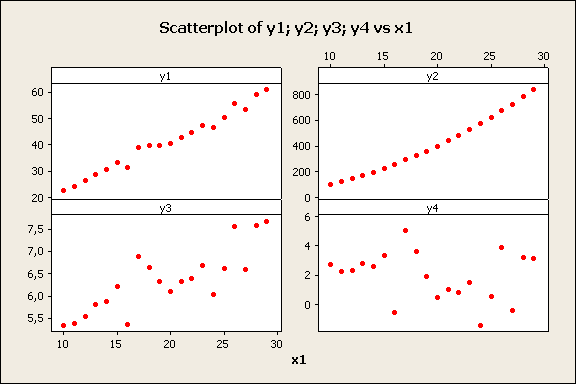
\includegraphics[scale=0.4]{6_9.png}}
      {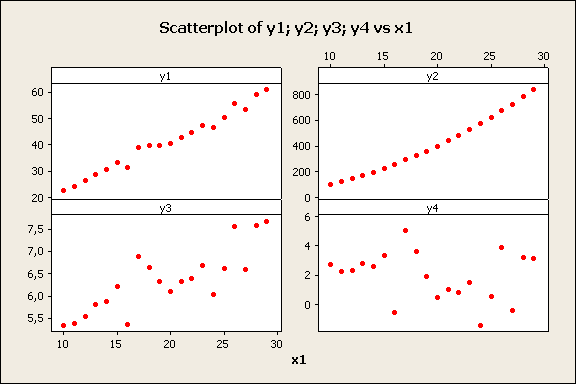
\includegraphics[scale=0.5]{6_9.png}}
  \end{center}
  An example of modeling choices is written in the examples of the plot. Each of the panel represents possible experimental relations among couples of variables.  
\end{frame}

\begin{frame}
  \vspace*{.2cm}
  \begin{small}
    \begin{itemize}
      \item $y1$ and $x$ show a couple of variables that can be modeled with a \textbf{linear trend}. However, in this kind of trend, there is a dispersion of data compared to the central trend. 
      \item $y2$ and $x$ show a couple of variables that can be well modeled with \textbf{parabolic} model. The functional link seems to be almost perfect.
      \item $y3$ and $x$ show a more uncertain relation between the couple of analysed variables, because the \textbf{effect of the residual variability} is really strong. It can be hypothesized both a linear relation, and a not linear relation between the data.
      \item Finally $y4$ and $x$ show an \textbf{almost random distribution} of the couples of the noticed observations.
      \item It is a researcher's task that of proving the different hypothesized functional relations and choosing the model that effectively represents the behavior of the phenomenon. 
    \end{itemize}
  \end{small}
\end{frame}



\livelloA{Linear and multiple regression analyis}

\livelloB{Linear regression analysis}

\begin{frame}
  \begin{itemize}
    \item If we want to study the relation between weight and height, it is possible to hypothesize that the weight is influenced by the height. In a regression model, the height is the independent variable and the weight is the dependent one.
    \item If $ y $ is the dependent variable and $ x $ the independent one, it is possible to write the relation like:
    \vspace{-0.4cm} $$ y_i = \beta_0 + \beta_1 \cdot x_i + \varepsilon_i $$ \vspace{-1cm} 
    \item Each observation $ y_i $ is characterised by a \textbf{deterministic element} (or structural element), $ f(x) = \beta_0 + \beta_1 \cdot  x_i $, and by a \textbf{random element}, $ \varepsilon_i $.
    \item The presence of the random element, $ \varepsilon_i $, makes the $ y_i $ random values. In other words, it is not possible to know exactly the value of $ y_i $, if we only know the value of $ x_i $.    
  \end{itemize}
\end{frame}

\begin{frame}
  \begin{itemize}
    \item As in the previous case, when the deterministic element is represented by a straight line, we talk about a \textbf{simple linear regression}. 
    \vspace{0.2cm}
    \item In the case of a simple linear regression:
    \begin{itemize}
      \item $ \beta_0 $ is the \textbf{intercept}, and it shows the $ y $ value when $ x $ is equal to $ 0 $;
      \item $ \beta_1 $ is the \textbf{slope} (or gradient), and it shows how much $ y $ changes when $ x $ increases in one unity.
    \end{itemize}
    \vspace{0.2cm}
    \item The plot in the following slide shows the geometrical meaning of the intercept and the slope of a line.
    \vspace{0.2cm}
    \item The line represented in the plot has an equation $ y = 40 + 15 \cdot x $.
  \end{itemize}
\end{frame}

\begin{frame}
  \begin{center}
    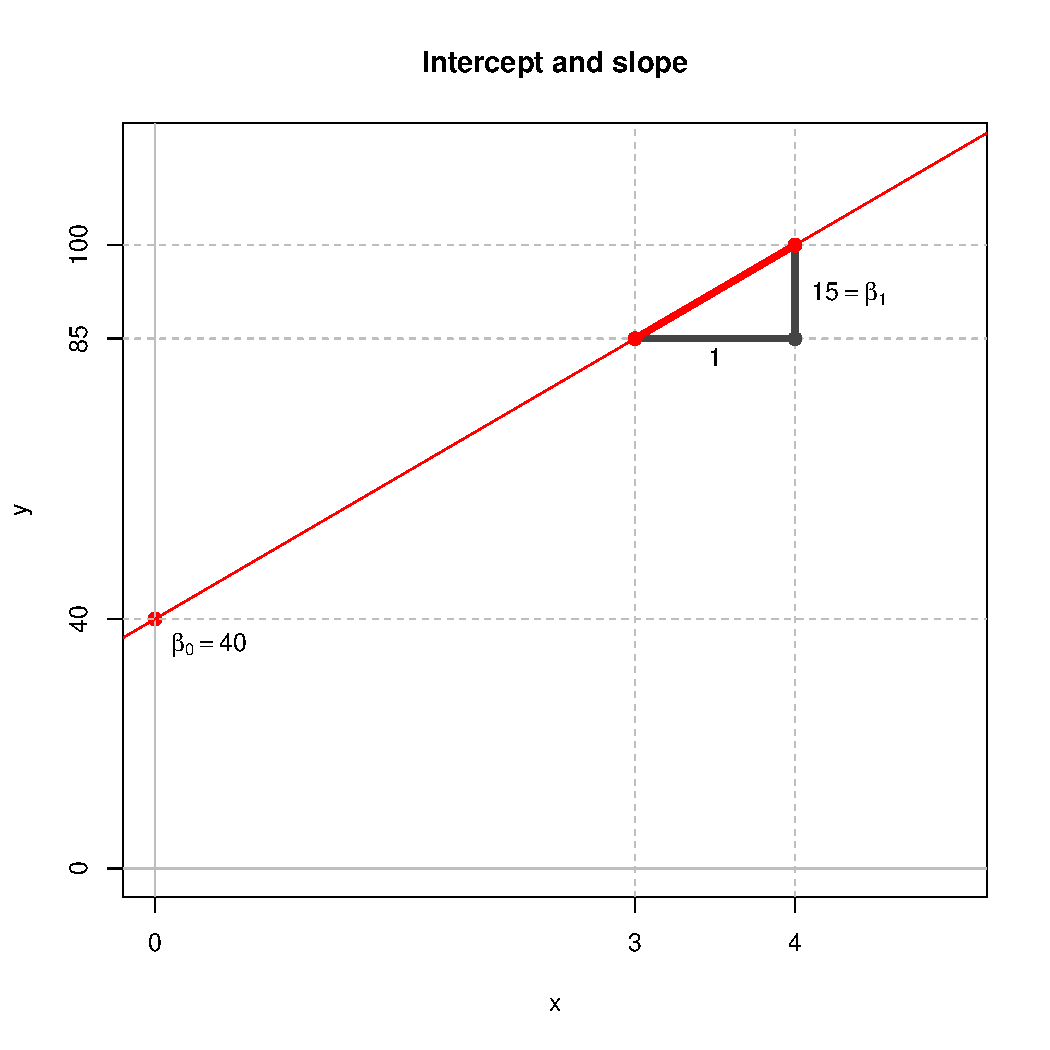
\includegraphics[scale=0.45]{6_interceptSlope.pdf}
  \end{center}
\end{frame}

\begin{frame}
  \begin{center}
    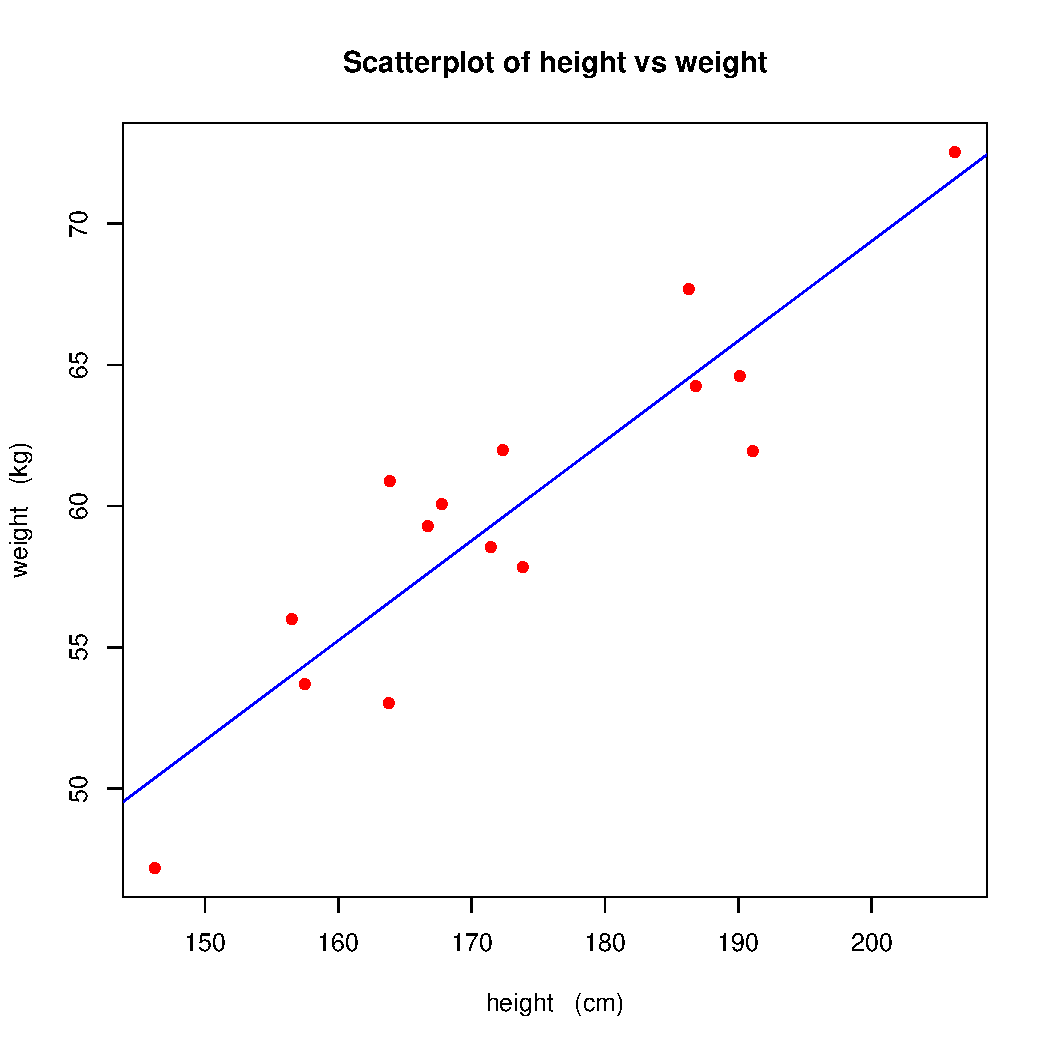
\includegraphics[scale=0.45]{6_scatt}
  \end{center}
\end{frame}

\begin{frame}
  \begin{itemize}
    \item The plot in the previous slide shows the weights and the corresponding height of $ n = 15 $ people. 
    \item The line represents the linear regression estimated between weight and height.
    \item The estimated regression line is the line that ``better crosses the points''.
    \item It is possible to write the estimated regression line's equation like $ \hat{y}_i = \hat{\beta_0} + \hat{\beta_1} \cdot x_i $ where $ \hat{\beta_0} $ and $ \hat{\beta_1} $ respectively represent the estimation of $ \beta_0 $ and $ \beta_1 $.
    \item The differences among the $ y_i $ observed values and the $ y_i $ estimated values through the regression line ($ \hat{y}_i $), are called \textbf{residuals}: \vspace{-0.5cm} $$ e_i = y_i - \hat{y}_i $$
  \end{itemize}
\end{frame}
    
\begin{frame}
  \vspace{0.25cm}
  \begin{itemize}
    \item How is it possible to obtain the estimations of $ \beta_0 $ and $ \beta_1 $, or rather those values for which the line ``better crosses the points''?
    \vspace{0.75cm}
    \item One of the most used criteria for the parameters' estimation ($ \hat{\beta_0} $ and $ \hat{\beta_1} $) of the regression model is the \textbf{ordinary least squares criterion}.
    \vspace{0.5cm}
    \item The ordinary least squares criterion finds the parameters of the curve that \textbf{minimize the sum of squared residuals}.
    \vspace{0.75cm}
    \item The next slides show three possible lines.
  \end{itemize}
\end{frame}

\begin{frame}
  \begin{center}
    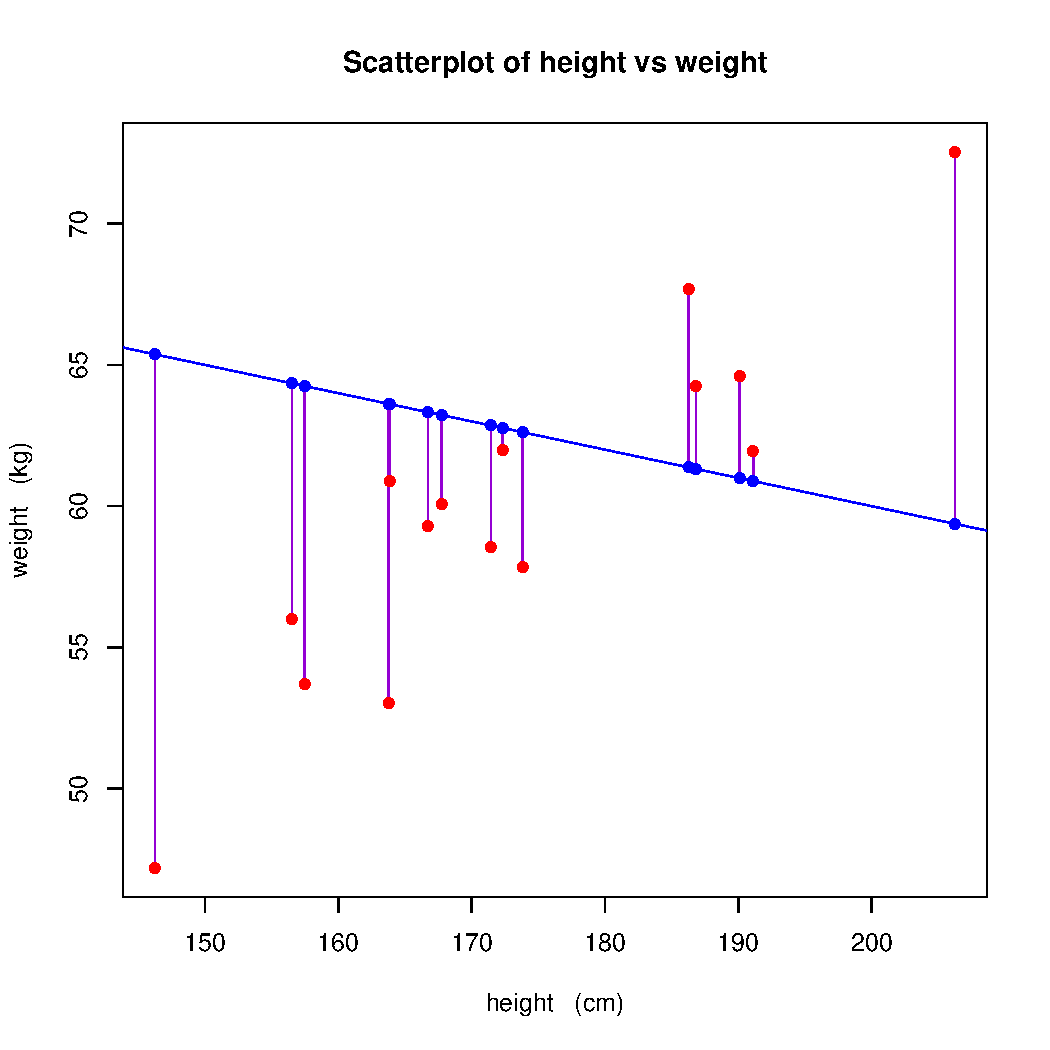
\includegraphics[scale=0.35]{6_scattErr}
  \end{center}
  \vspace{-0.4cm}
  \begin{small}
    The purple segments represent the residuals, or rather the differences between the true value of the weight (red points) and the estimated values of the lines (blue points).
  \end{small}
\end{frame}

\begin{frame}
  \begin{center}
    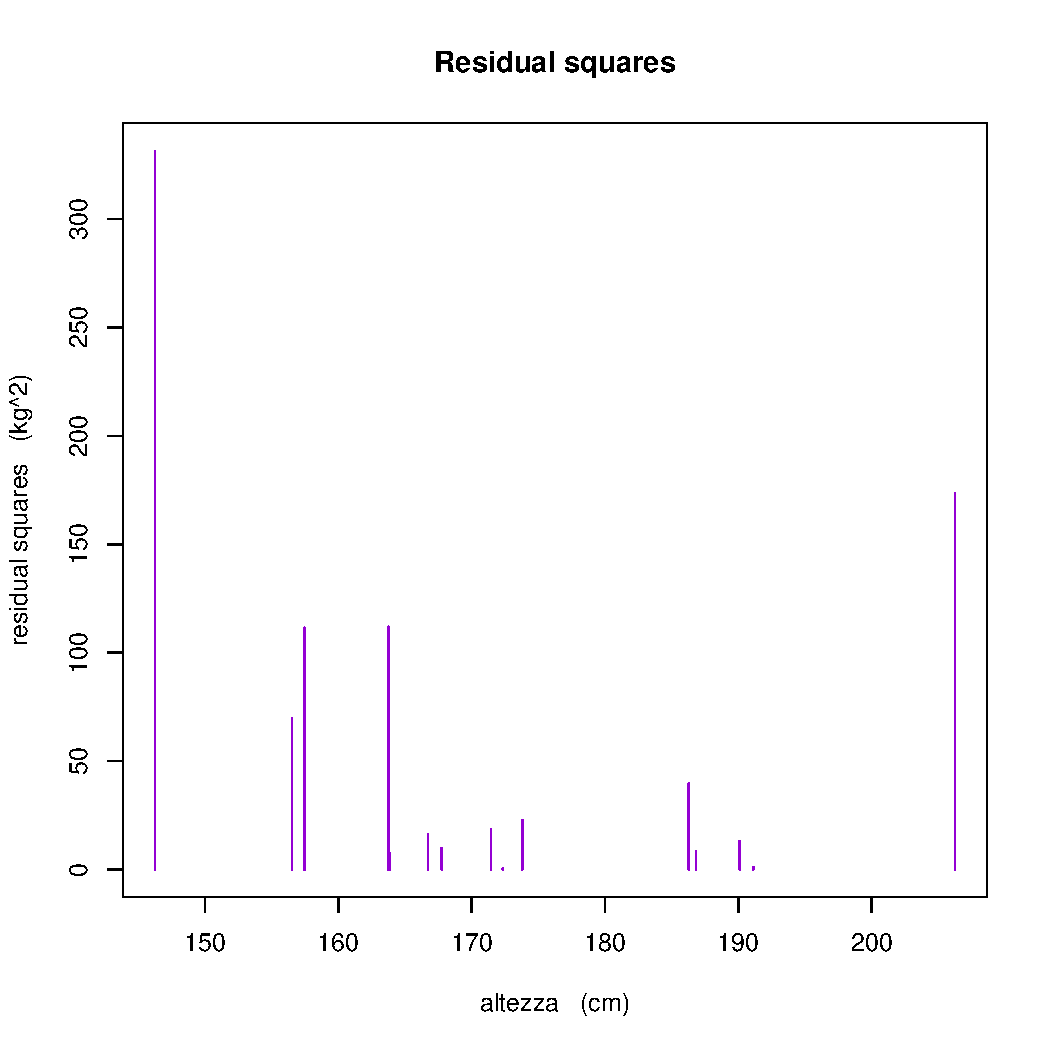
\includegraphics[scale=0.35]{6_scattErrSumSq}
  \end{center}
  \vspace{-0.4cm}
  \begin{small}
    The purple segments represent the squared residuals. \\
    The sum of squared residuals is 936.22.
  \end{small}
\end{frame}

\begin{frame}
  \begin{center}
    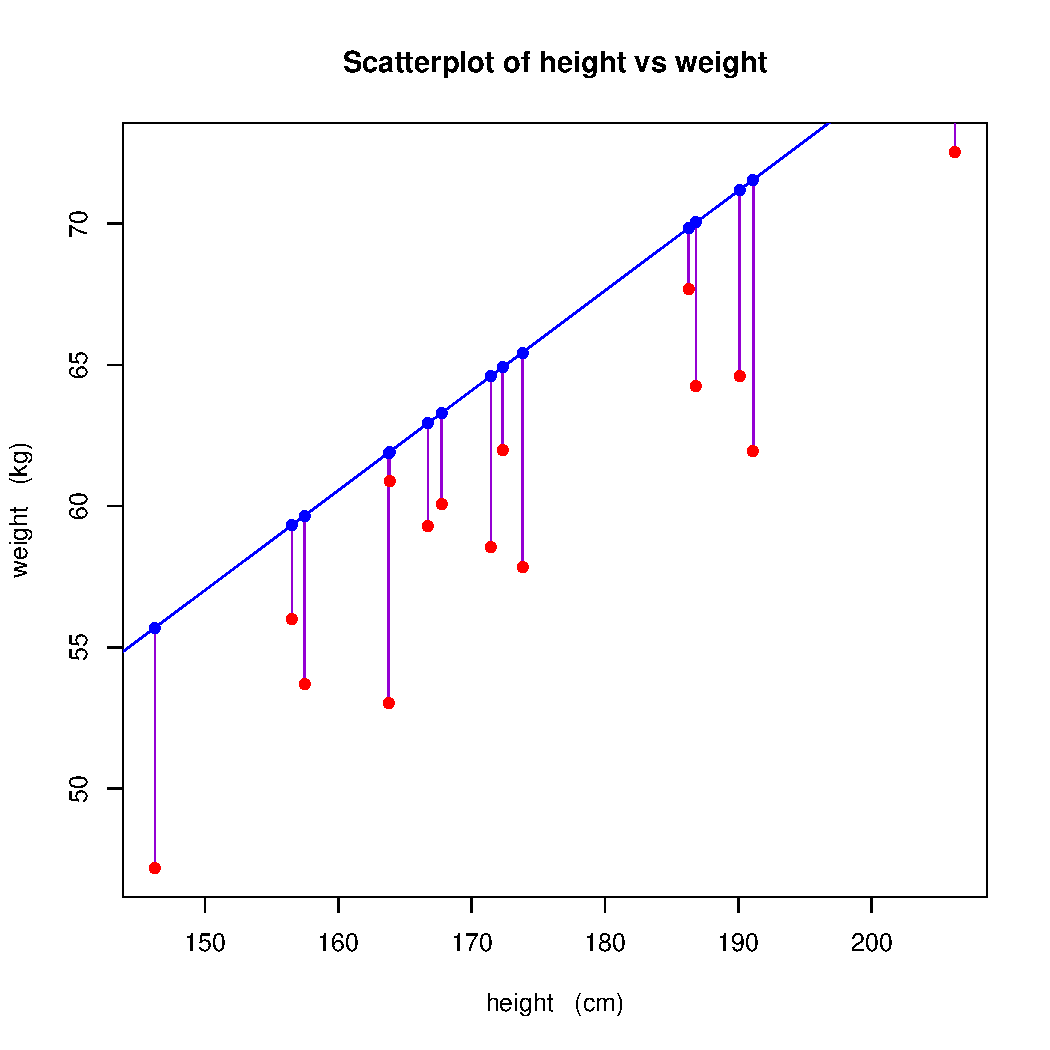
\includegraphics[scale=0.35]{6_scattInt}
  \end{center}
  \vspace{-0.4cm}
  \begin{small}
    The purple segments represent the residuals, or rather the differences between the true value of the weight (red points) and the estimated values of the lines (blue points).
  \end{small}
\end{frame}

\begin{frame}
  \begin{center}
    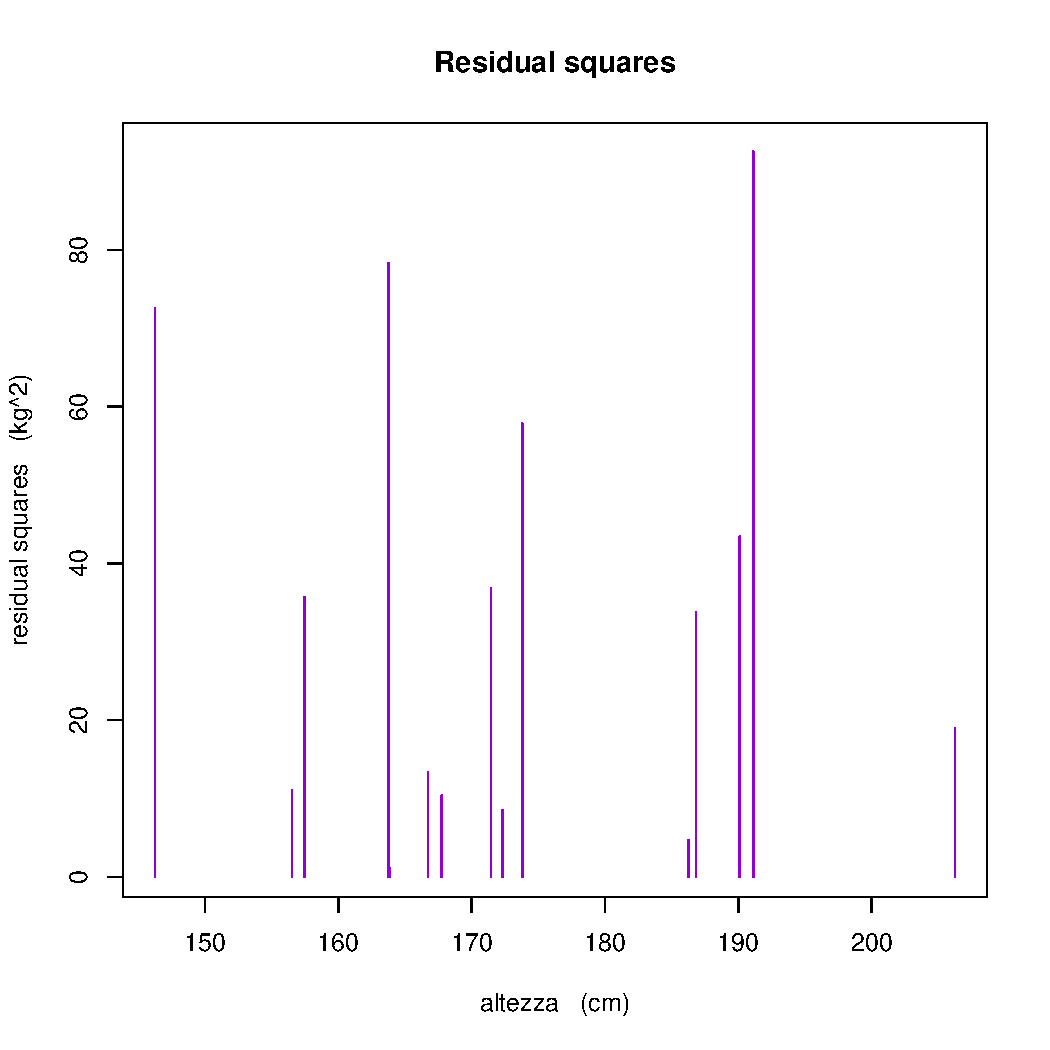
\includegraphics[scale=0.35]{6_scattIntSumSq}
  \end{center}
  \vspace{-0.4cm}
  \begin{small}
    The purple segments represent the squared residuals. \\
    The sum of squared residuals is 519.13.
  \end{small}
\end{frame}

\begin{frame}
  \begin{center}
    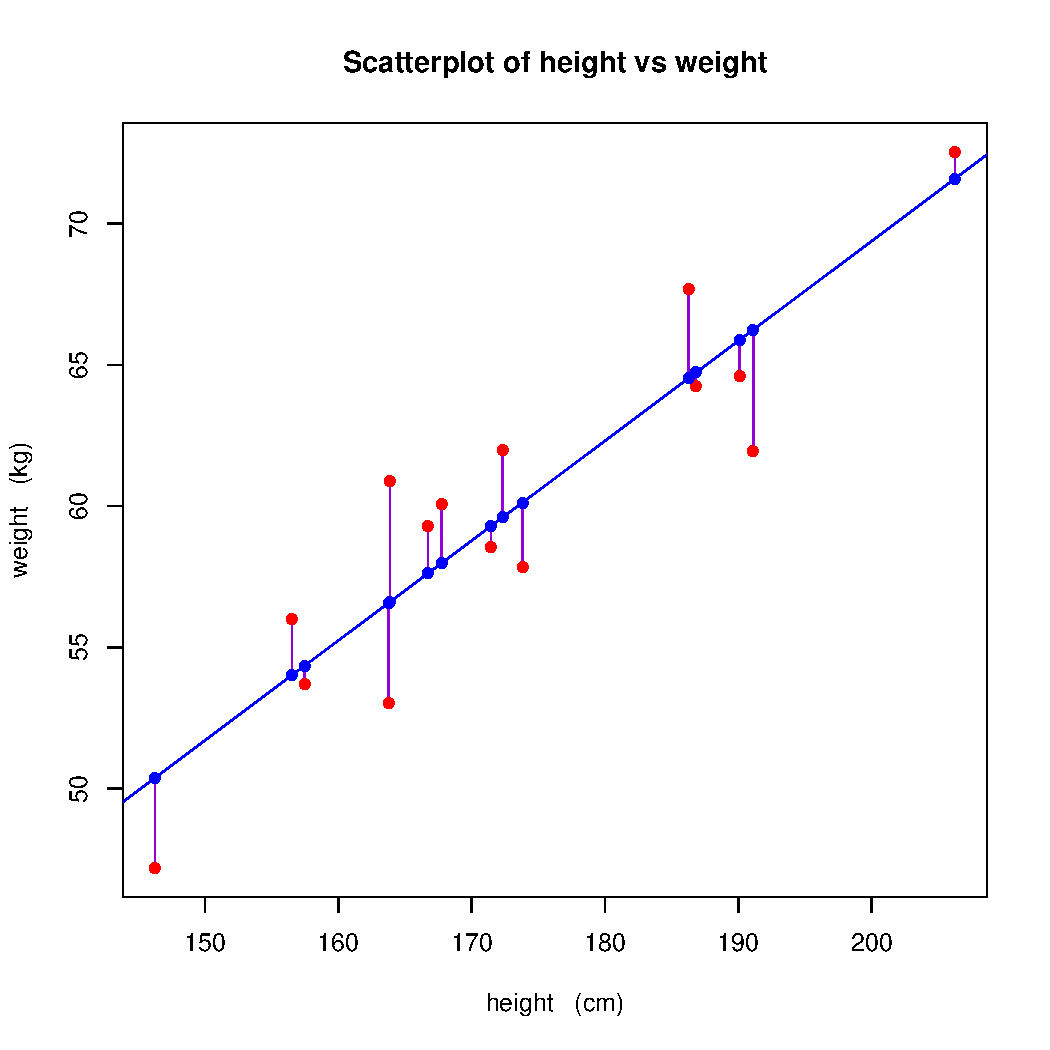
\includegraphics[scale=0.35]{6_scattMQ}
  \end{center}
  \vspace{-0.4cm}
  \begin{small}
    The purple segments represent the residuals, or rather the diffferences between the true value of the weight (red points) and the estimated values of the lines (blue points).
  \end{small}
\end{frame}

\begin{frame}
  \begin{center}
    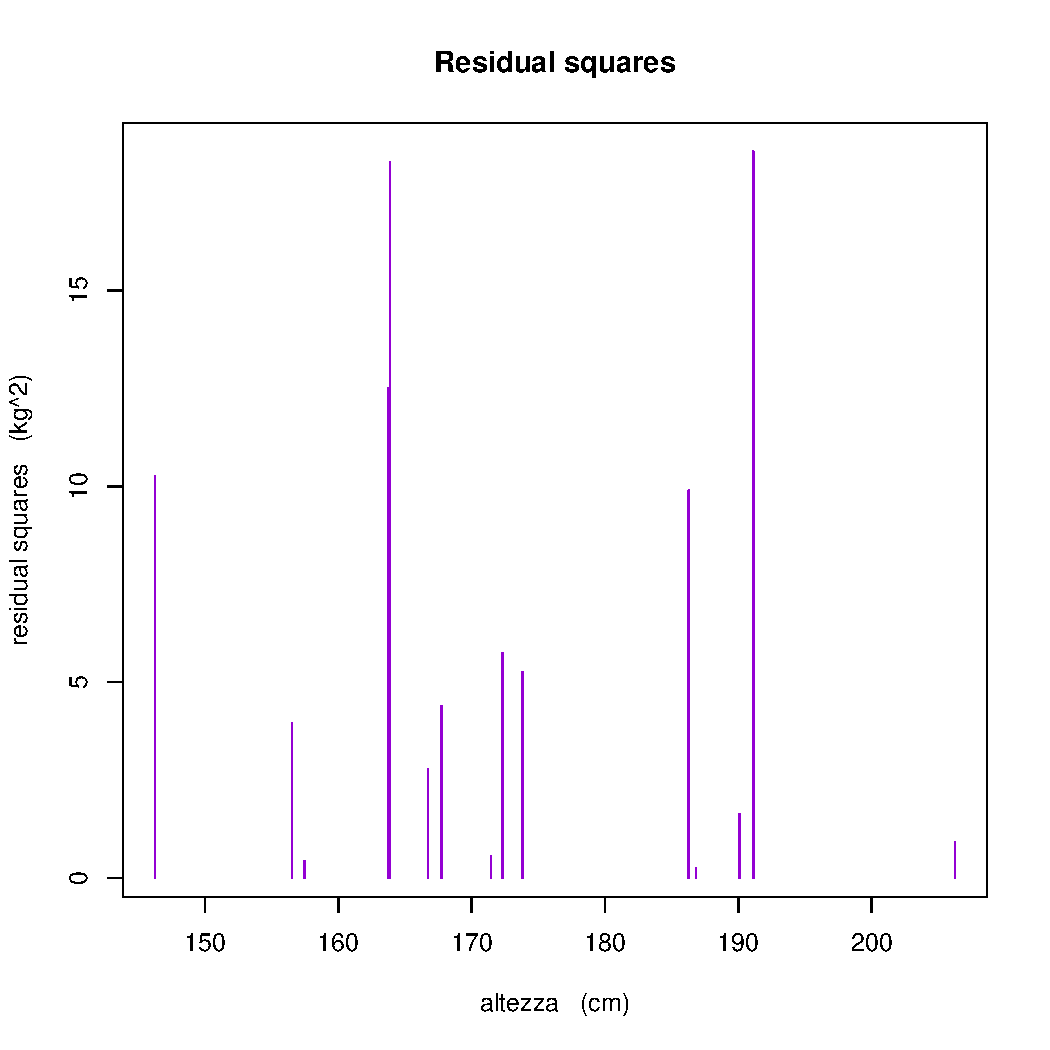
\includegraphics[scale=0.35]{6_scattMQSumSq}
  \end{center}
  \vspace{-0.4cm}
  \begin{small}
    The purple segments represent the squared residuals. \\
    The sum of squared residuals is 95.37.
  \end{small}
\end{frame}

\begin{frame}
  \vspace{0.25cm}
  \begin{itemize}
    \item From the previous plots it is possible to notice how the first two lines have a greater sum of squared residuals. On the contrary, the third one has a lower sum of squared residuals.
    \vspace{0.20cm}
    \item As a matter of fact, the first line has been calculated using random values for the intercept and the slope, that certainly do not ``better cross the points''.
    \vspace{0.20cm}
    \item In the second line it has been used the estimated value with the least squares method for the slope, and a random value for the intercept.
    \vspace{0.20cm}
    \item The third line is the regression one, estimated with the least squares method.
  \end{itemize}
\end{frame}

\begin{frame}
  \vspace{0.25cm}
  \begin{itemize}
    \item After having shown, in an intuitive way, what is the least squares method, we will briefly show its corresponding formula.
    \vspace{0.15cm}
    \item In mathematical words, we look for the values of $ \hat{\beta_0} $ and $ \hat{\beta_1} $ by which we have
      \vspace{-0.3cm} $$ (\hat{\beta_0}, \hat{\beta_1}) = \min_{\beta_0, \beta_1}\left\lbrace \sum_{i=1}^{n}{\left[ y_i-\left(\beta_0 + \beta_1 \cdot x_i \right) \right] ^2 }\right\rbrace $$ \vspace{-0.4cm}
    \vspace{0.15cm}
    \item After appropriate mathematical calculations, it is possible to find the formula that allows to calculate $ \hat{\beta_0} $ and $ \hat{\beta_1} $ :
      \vspace{-0.2cm} $$ \hat{\beta_0} = \bar{y} - \hat{\beta_1} \cdot \bar{x} $$
      $$ \hat{\beta_1} = \frac{\sum_{i=1}^n (x_i - \bar{x}) (y_i - \bar{y})}{\sum_{i=1}^n (x_i - \bar{x})^2} $$
  \end{itemize}
\end{frame}

\begin{frame}[label=stimaMQ]
  \begin{itemize}
    \item With the data we used in the plot and we wrote in the table of the following slide, we will find that  $ \hat{\beta_0} = -1.32 $ and $ \hat{\beta_1} = 0.35 $.
    \item The regression line represented in the graphic, is the line whose equation is $ y = -1.32 + 0.35 \cdot x $.
    \item As we said before, from the mathematical point of view, the \textbf{intercept} ($ \hat{\beta_0} $) represents the y value when x is equal to zero. \\ 
      The intercept does not often have a practical meaning, mainly when there are phisical measurements. \\
      In the example, it has no sense to think that the height can be equal to zero and then the weight can be negative.
    \item The \textbf{slope} ($ \hat{\beta_1} $) represents the (mean) growth of the y when an unit of x increases. In the example, it is possible to state that, when the height increases one centimeter, the weight increases $ 0.35 $ kilograms.
  \end{itemize}
\end{frame}

\begin{frame}
  \begin{center}
    \begin{footnotesize}
      \begin{tabular}{ccc}
        \hline
        $i$ & weight ($ y $) & height ($ x $) \\
        \hline
        1  & 60.08 & 167.75 \\
        2  & 57.83 & 173.80 \\
        3  & 59.29 & 166.74 \\
        4  & 61.94 & 191.12 \\
        5  & 64.24 & 186.84 \\
        6  & 72.55 & 206.25 \\
        7  & 58.54 & 171.44 \\
        8  & 67.68 & 186.28 \\
        9  & 53.69 & 157.47 \\
        10 & 47.18 & 146.25 \\
        11 & 60.89 & 163.88 \\
        12 & 53.04 & 163.77 \\
        13 & 62.00 & 172.33 \\
        14 & 64.61 & 190.10 \\
        15 & 56.00 & 156.51 \\
        \hline
        mean & 59.97 & 173.37 \\
      \end{tabular}
    \end{footnotesize}
  \end{center}
\end{frame}

\livelloB{Multiple linear regression analysis}

\begin{frame}
  \vspace{0.25cm}
  \begin{itemize}
    \item It has been considered the easiest case in which the dependent variable is the linear function of one independent variable so far. 
    \vspace{0.25cm}
    \item This regression model is called \textbf{simple linear regression model}.
    \vspace{0.25cm}
    \item The model often hypothesizes that the dependent variable is the linear function of more independent variables:
    \vspace{-0.4cm} $$ y_i = f(\vect{x_i}; \vect{\beta}) + \varepsilon_i = \beta_0 + \beta_1 \cdot x_{i1} + \beta_2 \cdot x_{i2} + \dots + \beta_p \cdot x_{ip} + \varepsilon_i $$\vspace{-1cm}
    \item[] where $ p $ represents the number of independent variables.
    \vspace{0.25cm}
    \item In this case the model is called \textbf{multiple linear regression model}.
  \end{itemize}
\end{frame}

\begin{frame}
  \vspace{0.25cm}
  \begin{itemize}
    \item Also in this case, for the estimation of the parameters $ \beta_j $, $ j = 0, 1, \dots, p $, the ordinary least squares method is used.
    \vspace{0.5cm}
    \item In mathematical words, the formulation of the estimation problem is similar to the previous one:
    \vspace{-0.3cm} $$\vect{\hat{\beta}} = \min_{\vect{\beta}}\left\lbrace \sum_{i=1}^{n}{\left[ y_i - f\left( \vect{x_i}; \vect{\beta} \right) \right]^2 }\right\rbrace $$\\
    \vspace{0.4cm}
    \item Similarly to the simple linear regression case, the \textbf{coefficients} $ \beta_j $ indicate the awaited variance of the response variable for an unitary increase of the relative explanatory variable $ x_j $, when the value of the other variables is constant.
  \end{itemize}
\end{frame}

\begin{frame}
  \vspace{0.25cm}
  \begin{itemize}
    \item In the previous slides it has been used the matrix notation too:
    \vspace{0.25cm}
    \begin{itemize}
      \item the vector $ \vect{y} $ represents the vector, with length $ n $, of the dependent variables;
      \vspace{0.25cm}
      \item the vector $ \vect{\beta} $ represents the vector, with length $ p + 1 $ (it is important to consider $ \beta_0 $), of the parameters that have to be estimated;
      \vspace{0.25cm}
      \item the matrix $ \matr{X} $ represents the matrix of the independent variables. 
      \vspace{0.25cm}
      \item the matrix $ \matr{X} $ has sizes $ n $ x $ (p + 1) $ and the first column contains all the values equal to 1. This column allows to calculate the value of the constant (or \textbf{intercept}).
      \vspace{0.25cm}
      \item The vector $ \vect{x_i} $ represents the $ i $th row of the matrix $ \matr{X} $.
    \end{itemize}
  \end{itemize}
\end{frame}

\livelloB{Polinomial regression analysis}

\begin{frame}
  As we have already seen in the slide about the functional relation, the relation between the x and the y can be not linear, as shown in the following graphic.
  \begin{center}
    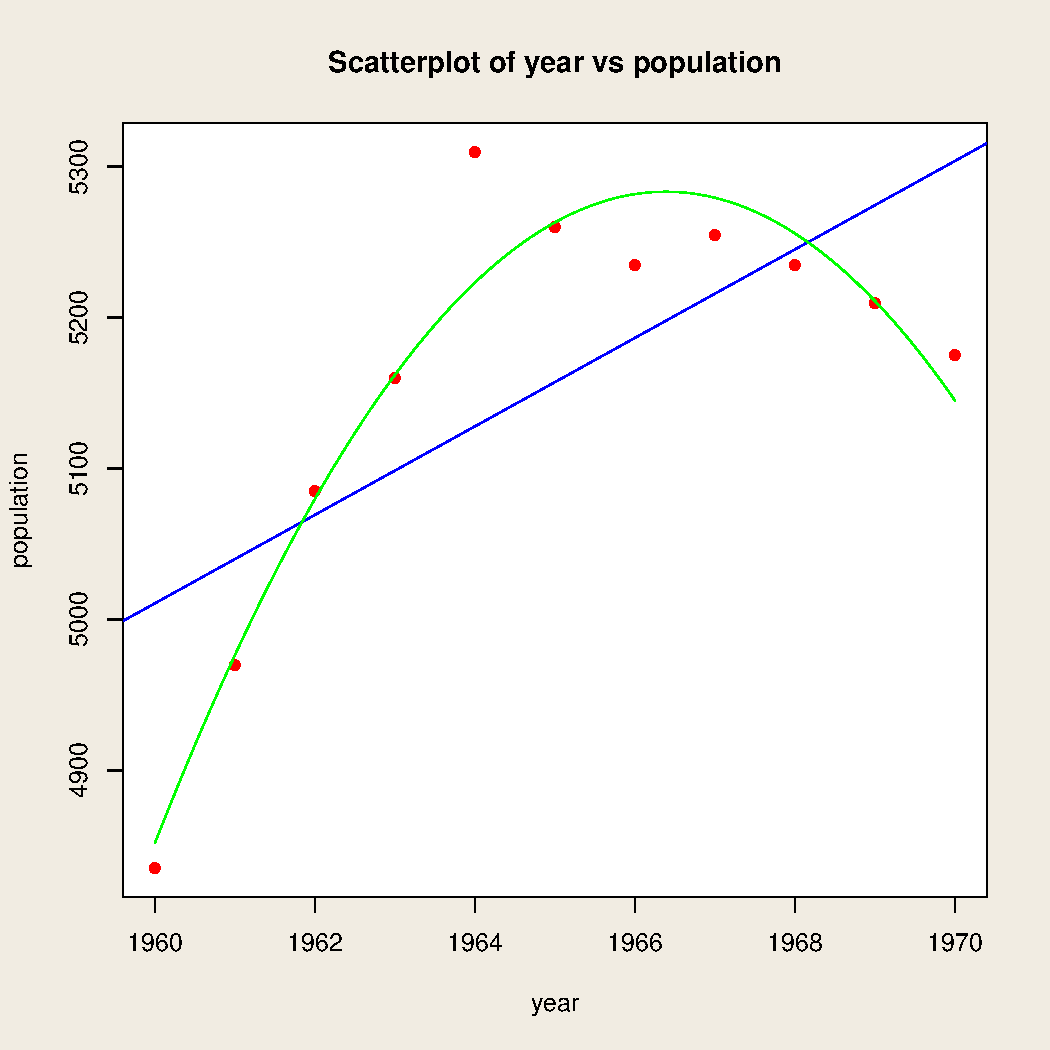
\includegraphics[scale=0.35]{6_polinom}
  \end{center}
\end{frame}

\begin{frame}
  \begin{itemize}
    \item The plot shows the population of a town in the 1960s.
    \item As we can see, the estimated linear regression, represented by the blue line, does not catch the relation between the x and the y.
    \item The parabola, the green one, seems to be better in catching this relation.
    \item In similar cases, it is possible to use a \textbf{quadratic regression} analysis, whose model can be formulated like
    \item[] \vspace{-0.6cm} $$ y_i = \beta_0 + \beta_1 \cdot x_{i1} + \beta_2 \cdot x_{i1}^2 + \varepsilon_i $$  \vspace{-0.8cm}
    \item This model, even though it is not linear in the variable, is \textbf{linear in the parameters}.
    \item As a matter of fact, if we consider that it is possible that $ x_{i2} = x_{i1}^2 $, this model can be considered as a particular case of a multivariate linear regression model.
  \end{itemize}
\end{frame}

\begin{frame}
  \vspace{0.25cm}
  \begin{itemize}
    \item Sometimes the polynomial can be a third degree one (\textbf{cubic regression}), or an higher degree one (\textbf{polinomial regression} of $ r $ degree).
    \vspace{0.15cm}
    \item Anyway, even though the model improves when the parameters increase, it is important to remember that a \textbf{parsimonious model}, or rather one with few parameters, is easiest to interpret.
    \vspace{0.15cm}
    \item Checking of the parameters' significance and using criteria such as the $ R^2 $ can help to choose the best model. These methods are described later.
    \vspace{0.15cm}
    \item Obviously, a polinomial model can include more variables, for example:
    \item[] \vspace{-0.6cm} $$ y_i = \beta_0 + \beta_1 \cdot x_{i1} + \beta_2 \cdot x_{i1}^2 + \beta_3 \cdot x_{i1}^3 + \beta_4 \cdot x_{i2} + \varepsilon_i $$ \vspace{-0.8cm}
  \end{itemize}
\end{frame}

\begin{frame}
  The plot shows how the relation between year and citrus fruits' production in Italy can be described by a cubic regression model. The green curve represents the curve $ y_i = \hat{\beta_0} + \hat{\beta_1} \cdot x_{i1} + \hat{\beta_2} \cdot x_{i1}^2 + \hat{\beta_3} \cdot x_{i1}^3 $. 
  \begin{center}
    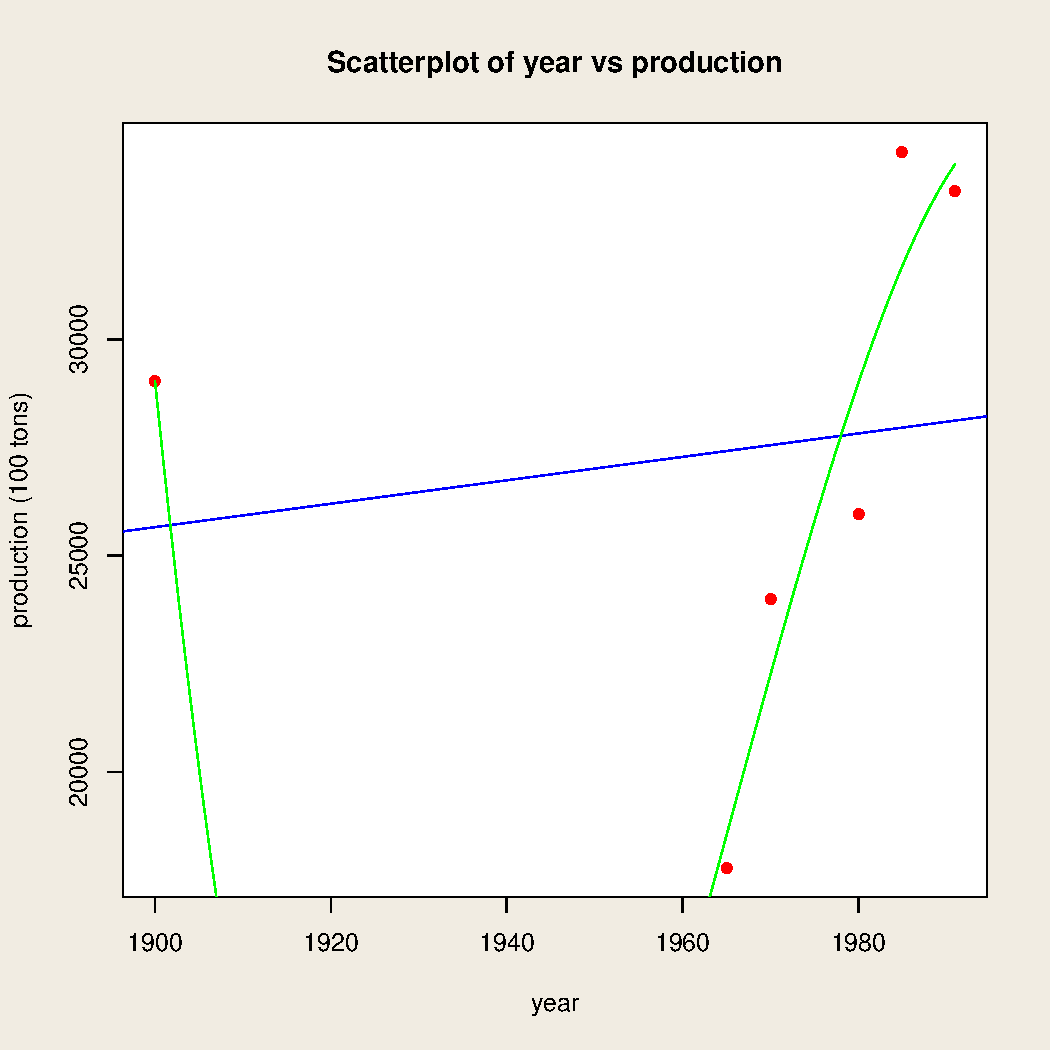
\includegraphics[scale=0.30]{6_cubic}
  \end{center}
  \vspace{-0.3cm}
  \begin{tiny}
    The example is taken by A. Quarteroni, F. Saleri, Calcolo Scientifico: Esercizi E Problemi Risolti Con Matlab E Octave, Springer
  \end{tiny}
\end{frame}

\livelloB[Interaction effects]{Interaction effects of the independent variables on the dependent one}

\begin{frame}
   \vspace*{.25cm}
  \begin{itemize}
    \item In some occasions, the relations that link the independent variables to the dependent one can be not ``released'' among them, but they can interact.
    \vspace{0.15cm}
    \item The synergic effect of the presence of two influent factors, can be ``depressive'' or ``explosive'' on the response variable.
    \vspace{0.15cm}
    \item For example, it is known that assuming alcohol together with drugs produces a synergic effect on the lucidity and the reactivity of a person. The synergic effect reduces the ability better than the sum of the effects.
    \vspace{0.15cm}
    \item In statistical and ``regression analysis'' words, this kind of effect, ``depressive'' or ``explosive'', is called \textbf{interaction effect} (or simply ``interaction'').
  \end{itemize}
\end{frame}

\begin{frame}
  \begin{center}
    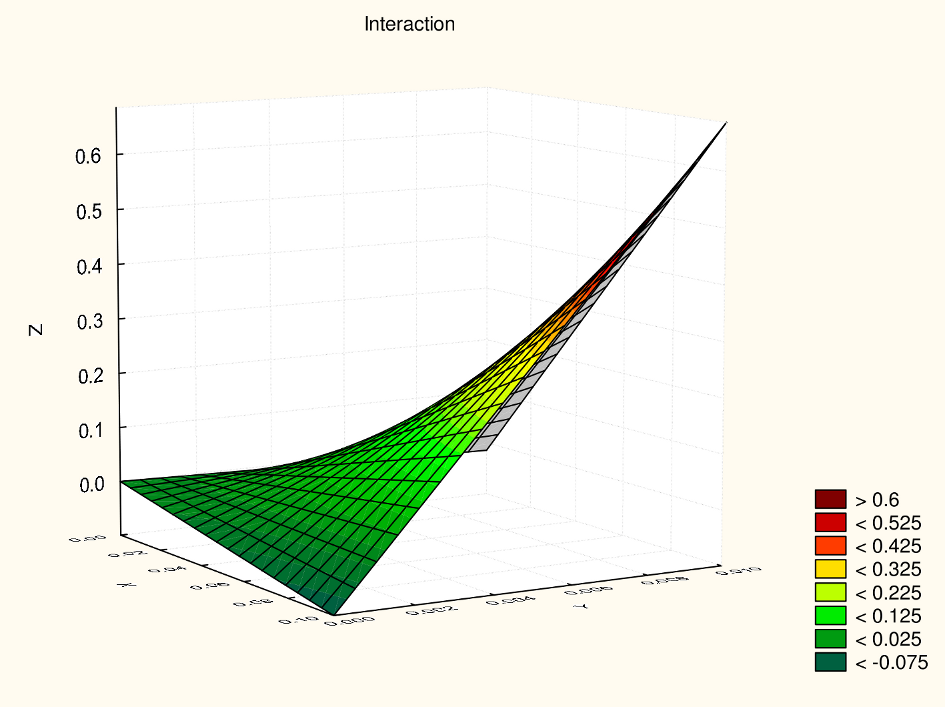
\includegraphics[scale=0.7]{6_regInteractionCont.png}
  \end{center}
  A plot example of an interaction effect between two continuous variables ($ x $ and $ y $) on the dependent variable ($ z $).
\end{frame}

\begin{frame}
  \vspace*{.25cm}
  \begin{itemize}
    \item It is possible that it is necessary to express the interaction effects among independent variables but we do not have specific information on the functional shape the relation has. In this case ``product'' operators are used. %, that links the independent variables with the dependent one,
    \vspace{0.25cm}
    \item For example, going back to the reaction times in function of the quantity of drug and alcohol assumed by a person, in order to express the joint relation of the explanatory variables (called $ x_1 $ e $ x_2 $) on the response variable($ y $), it can be used the following:
    \vspace{-0.3cm} $$ y_i = \beta_0 + \beta_1 \cdot x_{i1} + \beta_2 \cdot x_{i2} + \beta_3 \cdot x_{i1} \cdot x_{i2} + \varepsilon_i $$ \vspace{-1cm} \item[]
      where $ i $, $ i=1, \dots, n $, represents the $i$th sample observation.
  \end{itemize}
\end{frame}

\begin{frame}
  \vspace*{.5cm}
  \begin{itemize}
    \item The model can be elaborated and estimated by the creation of a third variable given by the row-by-row product of $ x_1 $ and $ x_2 $ values ($ x_{i3} = x_{i1} \cdot x_{i2} $) and then adding it to the model itself:\\
    \vspace{-0.4cm} $$ y_i = \beta_0 + \beta_1 \cdot x_{i1} + \beta_2 \cdot x_{i2} + \beta_3 \cdot x_{i3} + \varepsilon_i $$
    \vspace{0.5cm}
    \item At this point, the model can be estimated like a normal model of multiple regression.
  \end{itemize}
\end{frame}

\livelloB{Qualitative effects}

\begin{frame}
  \begin{small}
    \begin{itemize}
      \item Through the regression it is possible to analyse the qualitative effects on the response variable too.
      \item This is usually done using the \textbf{dummy variables}.
      \item The dummy variables (we will indicate them with the letter $ Z $) are (independent) variables that can assume only two values (0 o 1) and can be useful to indicate presence/lack of qualitative characteristics. The dummy variables conventionally:
      \vspace{-0.2cm}
      \begin{itemize}
        \item assume value \textbf{0} when the interest characteristic is \textbf{absent};
        \item assume value \textbf{1} when the interest characteristic is \textbf{present}.
      \end{itemize}
      \item The dummy variables are used also when a characteristic can assume just two different modalities, or rather where there are \textbf{dichotomous variables}. Some examples of these variables can be: male/female, minor/adult, employed/unemployed...\\
        In this case the choice to put a modality equal to 1 and the other equal to 0, or vice versa, is arbitrary and does not influence the results.
    \end{itemize}
  \end{small}
\end{frame}

\livelloB{Qualitative effects - Differences on the intercept}

\begin{frame}
  \vspace*{.25cm}
  \begin{itemize}
    \item It is supposed that we want to analyse the relation between height and weight of a series of people, distinguishing between males and females.
    \item It is hypothesized that the functional relation is locally linear and equal both for men and women, unless an intercept gap:
  \end{itemize}
  \begin{center}
    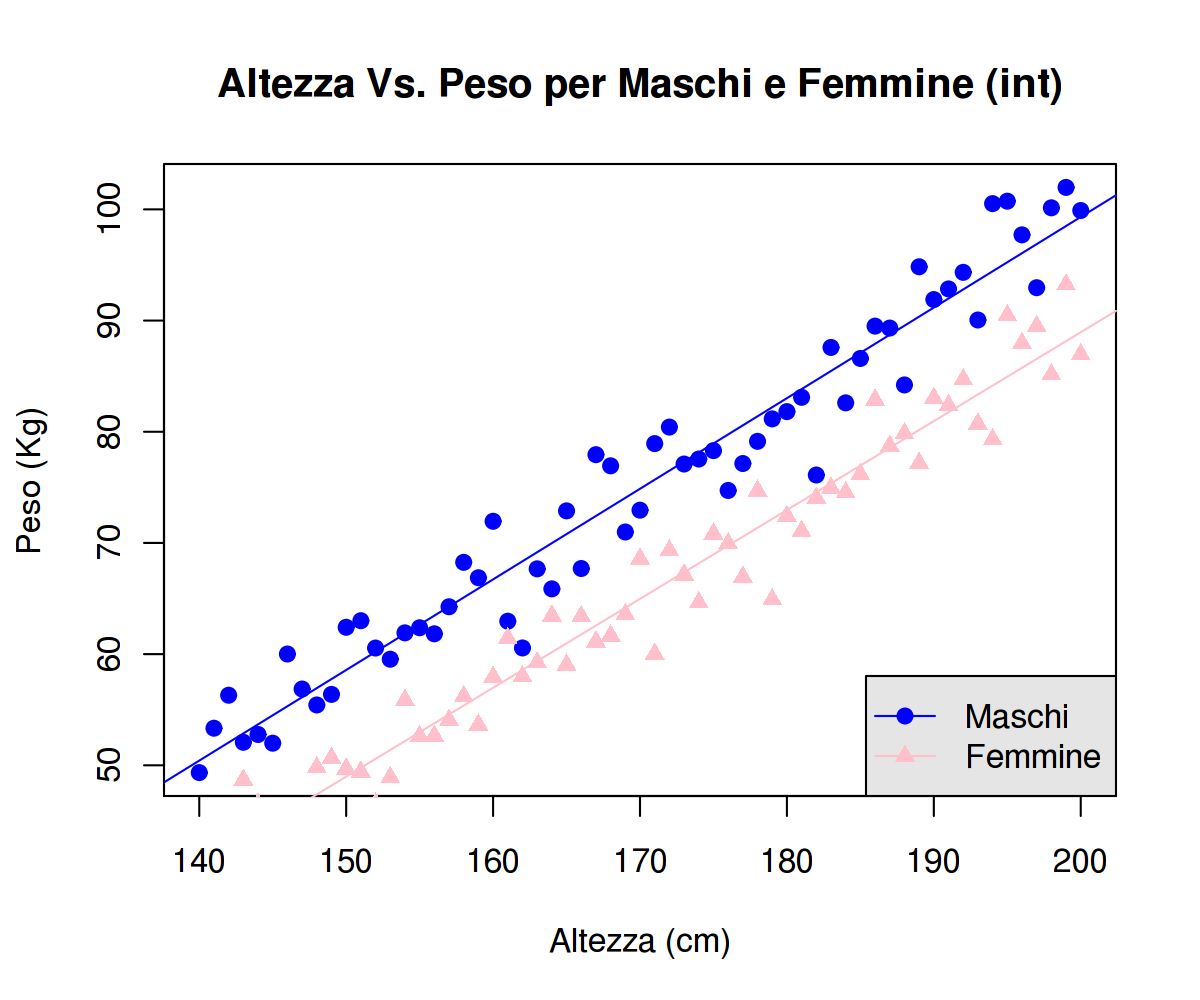
\includegraphics[scale=0.4]{6_regrIntercettaDiff.png}
  \end{center}
\end{frame}

\begin{frame}
  \vspace*{.25cm}
  \begin{itemize}
    \item It is possible to express in mathematical words this relation as a model like the following one:
    \vspace{-0.3cm} $$ y_i = \beta_0 + \beta_D \cdot Z_i + \beta_1 \cdot x_{i1} + \varepsilon_i $$\\
    \vspace{0.2cm}
    \item $Z_i$ is the dummy independent variable ``female'' that will have:
    \begin{itemize}
      \item value 0 if the $i$th subject is male;
      \item value 1 if the $i$th subject is female.
    \end{itemize}
    \vspace{0.25cm}
    \item $ \beta_D $ is the coefficient associated to the dummy variable that identifies the ``intercept gap'' between males and females.
  \end{itemize}
\end{frame}

\begin{frame}
  \vspace*{.25cm}
  \begin{itemize}
    \item If the subject is a male, as $ Z_i = 0 $, the model will be like:
    \vspace{-0.25cm} $$ y_i = \beta_0 + \beta_1 \cdot x_{i1} + \varepsilon_i = \beta_{0M} + \beta_1 \cdot x_{i1} + \varepsilon_i $$ \\
    \vspace{0.25cm}
    \item If the subject is a female, as $Z_i = 1$, the model will be like:
    \vspace{-0.50cm} $$ y_i = (\beta_0 + \beta_D) + \beta_1 \cdot x_{i1} + \varepsilon_i = \beta_{0F} + \beta_1 \cdot x_{i1} + \varepsilon_i $$ \\
    \vspace{0.25cm}
    \item As it can be noticed, the two models are almost identical, except for intercepts ($ \beta_{0M} $ and $ \beta_{0F }$) that will be different for males and females.
  \end{itemize}
\end{frame}

\begin{frame}
  \textbf{Example}. To study the linear relation between weight and height, according to the gender.\\
  \begin{center}
  \begin{tabular}{cccc}
    \hline
    \multicolumn{2}{c}{Men} & \multicolumn{2}{c}{Women} \\
    Height  & Weight     & Height  & Weight \\
    \hline
    167.8050 & 76.04820 & 162.2464 & 49.02631 \\
    174.5437 & 84.51962 & 159.5950 & 45.25246 \\
    175.9317 & 86.13436 & 164.6700 & 53.92118 \\
    175.3069 & 83.19130 & 174.5236 & 65.15938 \\
    177.6868 & 88.64845 & 162.6091 & 50.31901 \\
    170.0375 & 78.77422 & 162.9598 & 50.66751 \\
    173.8890 & 84.85968 & 165.0699 & 52.52929 \\
    180.0417 & 91.75516 & 162.4670 & 50.16048 \\
    170.7094 & 78.73333 & 165.4449 & 56.30775 \\
    174.7580 & 82.41510 & 165.6076 & 55.06725 \\
    \hline
  \end{tabular}
  \end{center}
\end{frame}

\begin{frame}
  The following plot shows the data.
  \begin{center}
    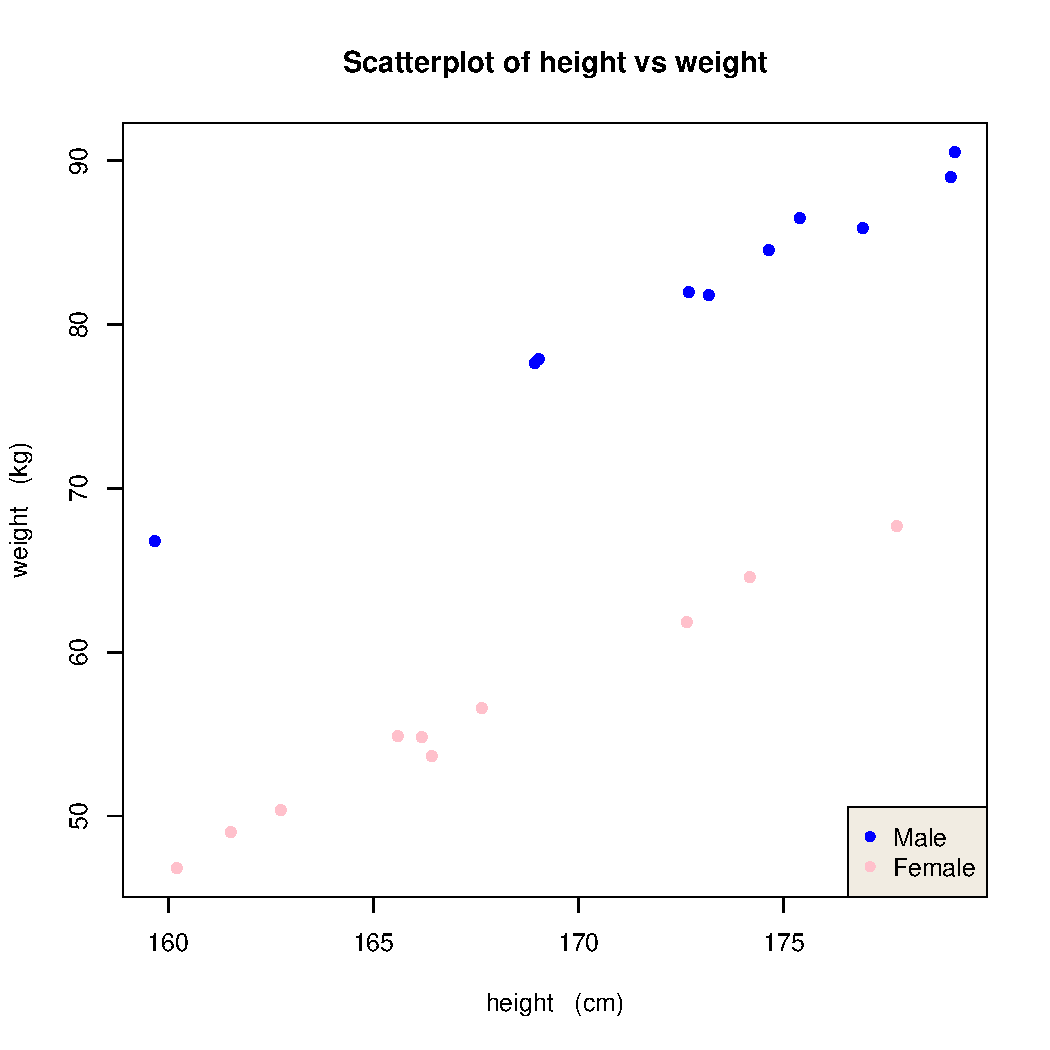
\includegraphics[scale=0.40]{6_qualitativiIntercetta}
  \end{center}
\end{frame}

\begin{frame}
  The estimated model can be expressed like: $$ \hat{y}_i = \hat{\beta}_0 + \hat{\beta}_1 \cdot x_{i} + \hat{\beta}_2 \cdot Z_{i} $$ where $ \hat{y}_i $ is the weight estimated value by the regression of the $i$th subject, $ \hat{\beta}_0 $ and the intercept for the women, $ \hat{\beta}_1 $ is the coefficient associated to the height ($ x_{i} $) and $ \hat{\beta}_2 $ is the estimation of the difference between men and women weight.\\
  \vspace{1cm}
  \begin{center}
    \begin{tabular}{|l|c|c|c|c|}
      \hline
                 &       estimate & Std. Error & t value & Pr($>|$t$|$)\\ 
      \hline
      Intercept & -141.53018 &    4.82671 &  -29.32 &   5.35e-16  \\
      \hline
      x          &    1.17950 &    0.02879 &   40.97 &   $<$ 2e-16   \\
      \hline
      Z          &   19.88756 &    0.35212 &   56.48 &   $<$ 2e-16   \\
      \hline
    \end{tabular}
  \end{center}
\end{frame}

\begin{frame}[fragile]
  The plot shows the data and the regression lines that have just been estimated.
  \begin{center}
    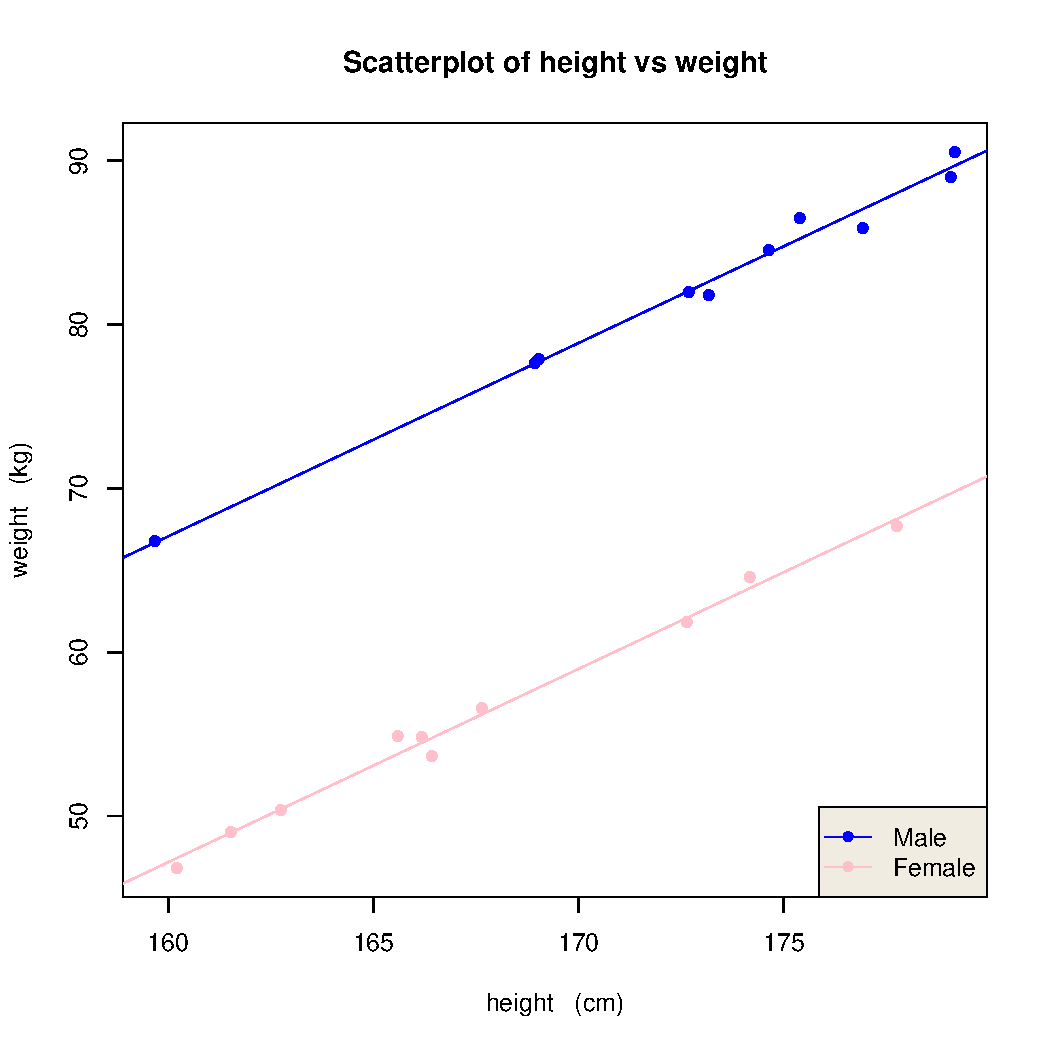
\includegraphics[scale=0.40]{6_qualitativiIntercettaRegr}
  \end{center}
\end{frame}

\livelloB{Qualitative effects - Differences on/of slope}

\begin{frame}
  \begin{itemize}
    \item If we want to analyse, in this case too, the relation between height and weight of a series of subjects, distiguishing between males and females.
    \item If we hypothesize that the functional relation is locally linear and equal both for males and females, unless a slope gap:
  \end{itemize}
  \begin{center}
    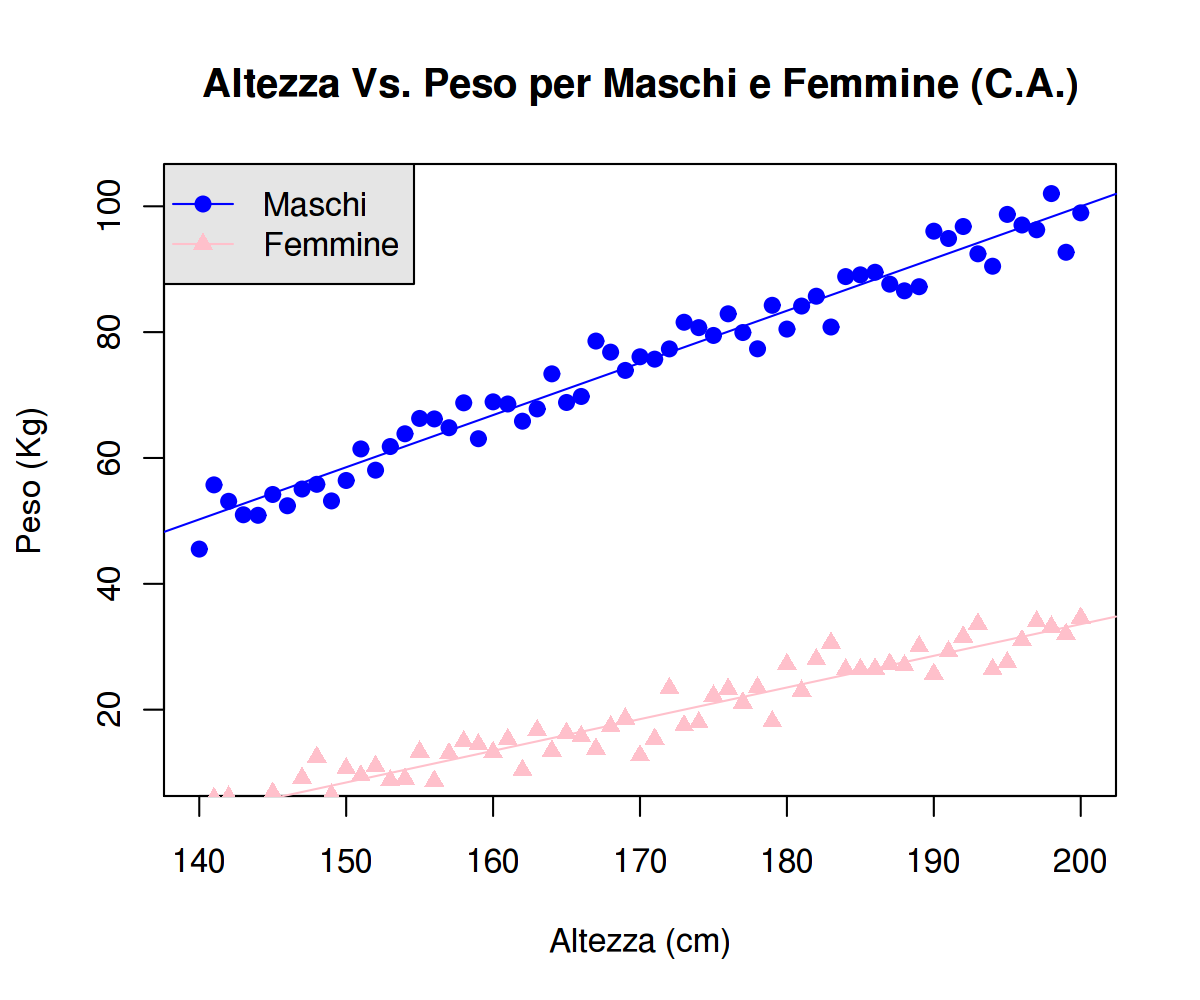
\includegraphics[scale=0.4]{6_regrCADiff.png}
  \end{center}
\end{frame}

\begin{frame}
  \vspace*{.25cm}
  \begin{itemize}
    \item It is possible to express this relation in mathematical words with a model like the one that follows:
    \vspace{-0.3cm} $$y_i = \beta_0 + \beta_D \cdot Z_i \cdot x_{i1} + \beta_1 \cdot x_{i1} + \varepsilon_i $$\\
    \vspace{0.2cm}
    \item $Z_i$ is the dummy independent variable ``female'' that will have:
    \begin{itemize}
      \item value 0 if the $i$th subject is male;
      \item value 1 if the $i$th subject is female.
    \end{itemize}
    \vspace{0.25cm}
    \item $ \beta_D $ is the coefficient associated to the dummy variable that identifies the ``slope gap'' between males and females.
  \end{itemize}
\end{frame}

\begin{frame}
  \vspace*{.25cm}
  \begin{itemize}
    \item If the subject is a male, as $ Z_i= 0 $, the model is like:
      \vspace{-0.25cm} $$ y_i = \beta_0 + \beta_1 \cdot x_{i1} + \varepsilon_i = \beta_0 + \beta_{1M} \cdot x_{i1} + \varepsilon_i $$ \\
    \vspace{0.25cm}
    \item If the subject is a female, as $ Z_i=1 $, the model is like:
      \vspace{-0.5cm} $$ y_i = \beta_0 + (\beta_D + \beta_1) \cdot x_{i1} + \varepsilon_i = \beta_0 + \beta_{1F} \cdot x_{i1} + \varepsilon_i$$ \\
    \vspace{0.25cm}
    \item As we can notice, the two models are almost identical, except for slopes ($\beta_{1M}$ and $\beta_{1F}$), that will be different for males and females.
\end{itemize}
\end{frame}

\livelloB{Qualitative effects - Differences on intercept and slope}

\begin{frame}
  \begin{itemize}
    \item If we want to analyse the relation between height and weight of a series of subject, distinguishing between males and females. 
    \item If it is hypothesized that the functional relation is locally linear and equal to males and females, unless a slope and an intercept gaps:
  \end{itemize}
  \begin{center}
    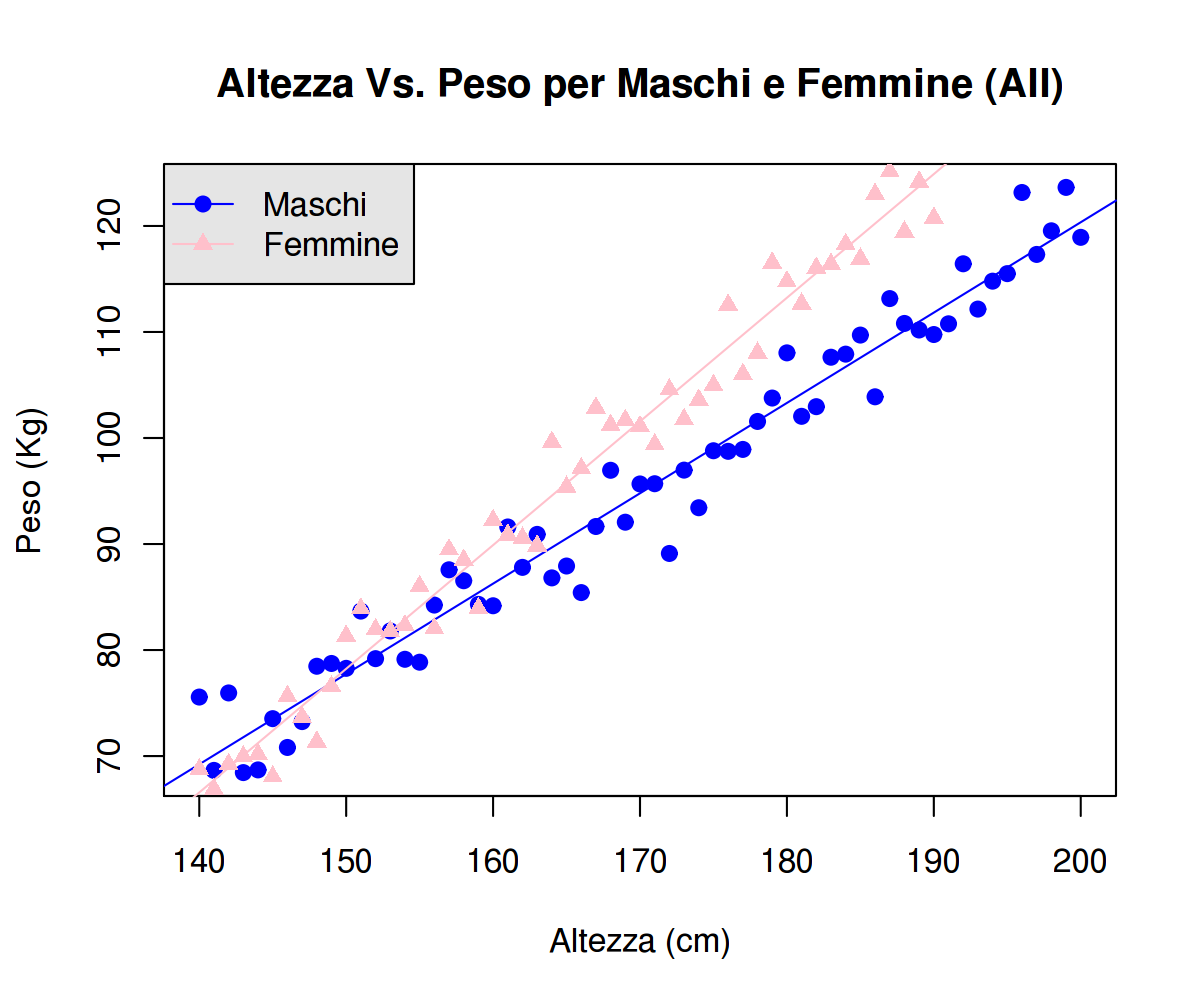
\includegraphics[scale=0.4]{6_regrAllDiff.png}
  \end{center}
\end{frame}

\begin{frame}
  \vspace*{.25cm}
  \begin{itemize}
    \item It is possible to express this relation in mathematical words with a model like the one that follows:
      \vspace{-0.3cm} $$ y_i = \beta_0 + \beta_{0D} \cdot Z_i + \beta_{1D} \cdot Z_i \cdot x_{i1} + \beta_1 \cdot x_{i1} + \varepsilon_i $$ 
    \item $Z_i$ is the independent dummy variable ``female'' that will have:
    \begin{itemize}
      \item value 0 if the $i$th subject is a male;
      \item value 1 if the $i$th subject is a female.
    \end{itemize}
    \vspace{0.2cm}\item $ \beta_{0D} $ is the coefficient associated to the dummy variable that identifies the ``intercept gap'' between males and females.
    \item $ \beta_{1D} $ is the coefficient associated to the dummy variable that identifies the ``slope gap'' between males and females.
  \end{itemize}
\end{frame}

\begin{frame}
  \vspace*{.25cm}
  \begin{itemize}
    \item If the subject is a male, as  $ Z_i=0 $, the model will be:
      \vspace{-0.25cm} $$ y_i = \beta_0 + \beta_1 \cdot x_{i1} + \varepsilon_i = \beta_{0M} + \beta_{1M} \cdot x_{i1} + \varepsilon_i $$ \\
    \vspace{0.25cm}
    \item If the subject is female, as $ Z_i=1 $, the model will be:
      \vspace{-0.5cm} $$ y_i= (\beta_0 + \beta_{0D}) + (\beta_{1D} + \beta_1) \cdot x_{i1} + \varepsilon_i = \beta_{0F} + \beta_{1F} \cdot x_{i1} + \varepsilon_i $$ \\
    \vspace{0.25cm}
    \item As we can noticed, the two model will be different because of both the intercepts ($ \beta_{0M} $ e $ \beta_{0F} $) and the slopes ($ \beta_{1M} $ e $ \beta_{1F} $), that will be different for males and females.
  \end{itemize}
\end{frame}

\livelloB[Qualitative effects - Multicategorical variables]{Qualitative effects - Extension to the case of multicategorical variables}

\begin{frame}
  \vspace{0.25cm}
  \begin{itemize}
    \item The use of the dummy variables is really flexible. It allows to build even complex models.
    \vspace{0.25cm}
    \item It has to be noticed, for example, that the use of dummy can be extended to the case of qualitative variables that can have more than two modalities (for example: income brackets, colors, used materials etc.).
    \vspace{0.25cm}
    \item If we want to analyse the relation between weight and height of a series of subjects, distinguishing them according to the continent they come from, it is possible to consider five different dummy variables. Each of these variables is equal to 1 if the subject comes from that continent and 0 if he does not. 
  \end{itemize}
\end{frame}

\begin{frame}
  \begin{itemize}
    \item In the practice, the construction of the dummy variables is delegated to the statistical analysis' softwares that make the work easier.
    \item It has to be noticed that, when we study the results given by the software, the dummy variables that have been used will be one less than the categorical variables modalities, e.g. than the number of continents. 
    \item In the case of the differences between males and females we saw in the previous examples, the dummy regarded just the ``female'' and the corresponding coefficients indicated the gaps compared to the``male''.
    \item Similarly, in the case of the continents, the dummy only regards four continents and the corresponding coefficients will indicate the gaps compared to the fifth continents, considered the reference one.
  \end{itemize}
\end{frame}

\livelloB{Linearizable models}

\begin{frame}
  \vspace{0.25cm}
  \begin{itemize}
    \item Sometimes it can happen that the relation between the dependent variable and the independent variables is not linear even in the parameters.
    \vspace{0.25cm}
    \item Sometimes it is possible that a not linear model in the parameters can be transformed in a linear one with appropriate transformations.
    \vspace{0.25cm}
    \item An exhaustive report of the different situations where the not linear model can be linearised is not possible in this course.
    \vspace{0.25cm}
    \item We will following give an example with two models: one that cannot be linearised and another that, on the contrary, can be linearised. 
  \end{itemize}
\end{frame}

\begin{frame}
  \vspace{0.25cm}
  \begin{itemize}
    \item It is supposed that the relation is expressed by functions like $ y_i = \beta_0 \cdot e^{\beta_1 \cdot x_i} + \varepsilon_i $ or $ y_i = \beta_0 \cdot e^{\beta_1 \cdot x_i} \cdot \varepsilon_i $.
    \vspace{0.25cm}
    \item The two models distinguish one from the other by the relationship, respectively additive and multiplicative, of the error term.
    \vspace{0.25cm}
    \item The following slide shows two plots, one with the additive error term, where the confidence bands are equidistant to the regression curve, and the other one with the multiplicative error term, where the confidence bands detach themselves when x increases.
  \end{itemize}
\end{frame}

\begin{frame}
  \begin{center}
    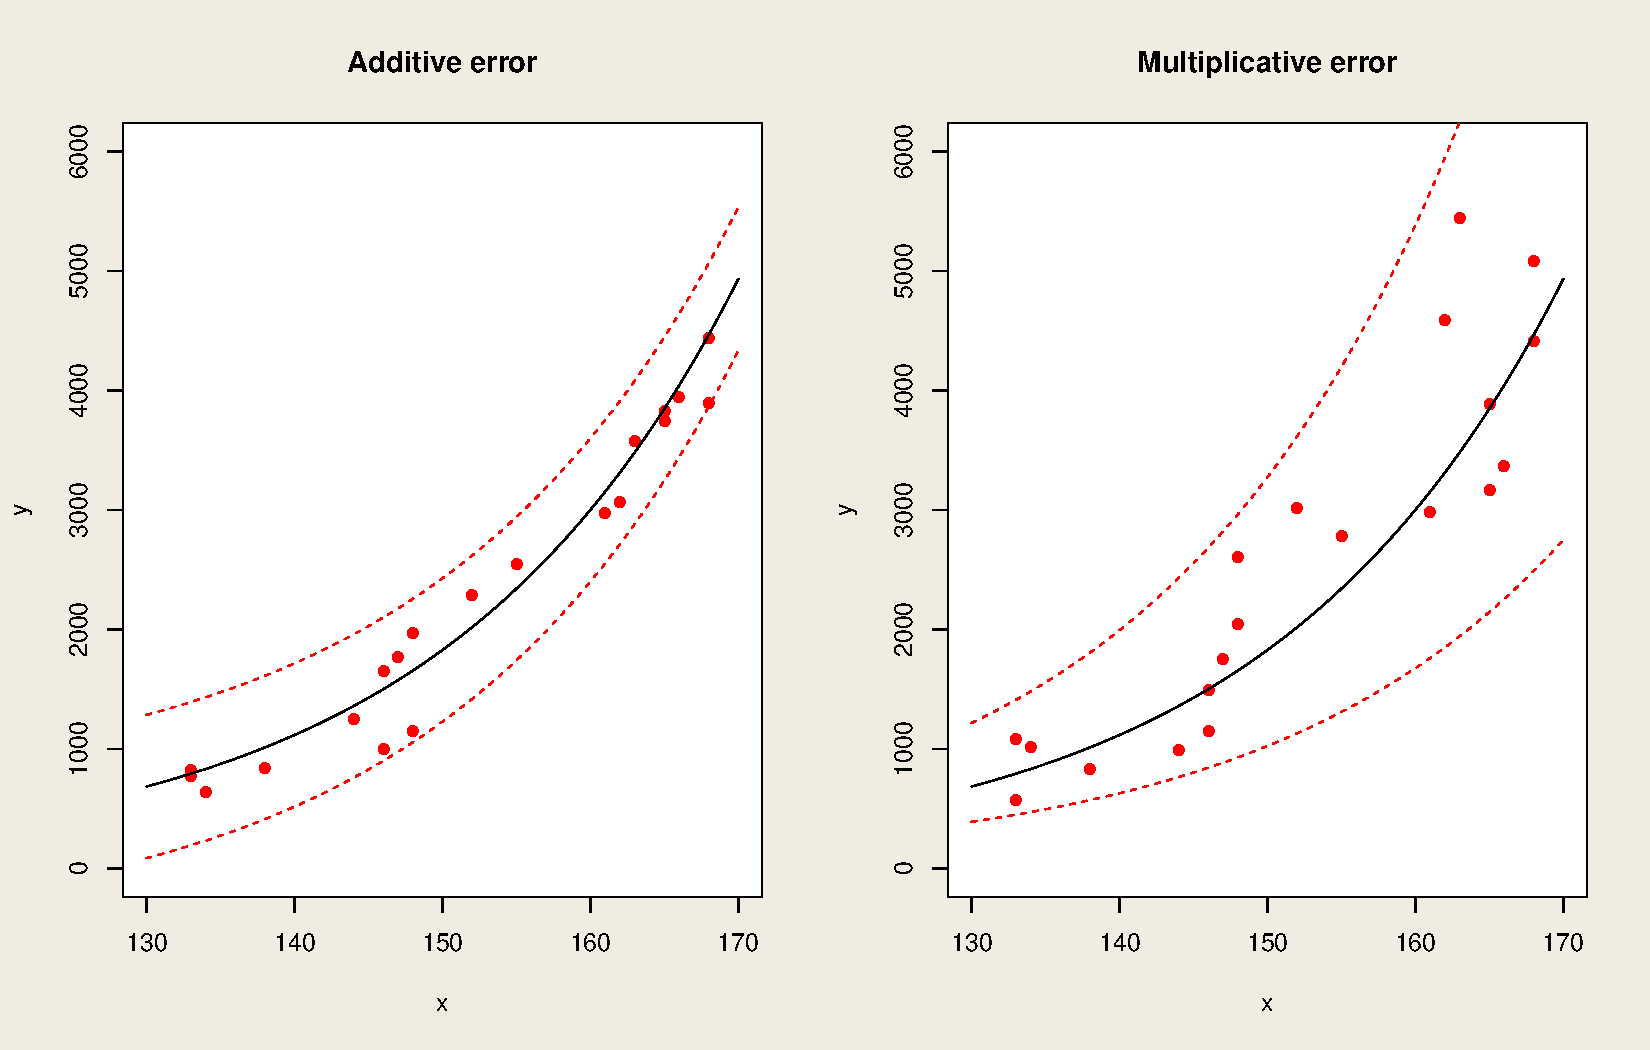
\includegraphics[scale=0.40]{6_exp}
  \end{center}
\end{frame}

\begin{frame}
  \begin{itemize}
    \item The first case requires the use of not linear techniques in order to find the regression curve.
    \item The second case, thanks to the logarithm characteristics, allows to lead to a linear model.
    \vspace{-0.5cm}
    \begin{displaymath}
      \begin{split}
        y_i &= \beta_0 \cdot e^{\beta_1 \cdot x_i} \cdot \varepsilon_i \\
        \ln(y_i) &= \ln(\beta_0 \cdot e^{\beta_1 \cdot x_i} \cdot \varepsilon_i) \\
        y_i^* &= \beta_0^* + \beta_1 \cdot x_i + \varepsilon_i^*
      \end{split}
    \end{displaymath}
    \item The parameters estimations are: $ \hat{y_i} = e^{\hat{y_i}^*} $, $ \hat{\beta_0} = e^{\hat{\beta_0}^*} $ and $ \hat{\varepsilon_i} = e^{\hat{\varepsilon_i}^*} $.
    \item It has to be noticed that $ \hat{y_i}^* $ is a not distorted estimator of $ y_i^* $, but $ \hat{y_i} $ it is not a not distorted estimator of $ y_i $.
    \item Furthermore, as for the hypothesis of the linear model $ \varepsilon_i^* $ has to have a normal distribution, then $ \varepsilon_i $ has to have a lognormal distribution.
  \end{itemize}
\end{frame}

\begin{frame}
  \begin{center}
    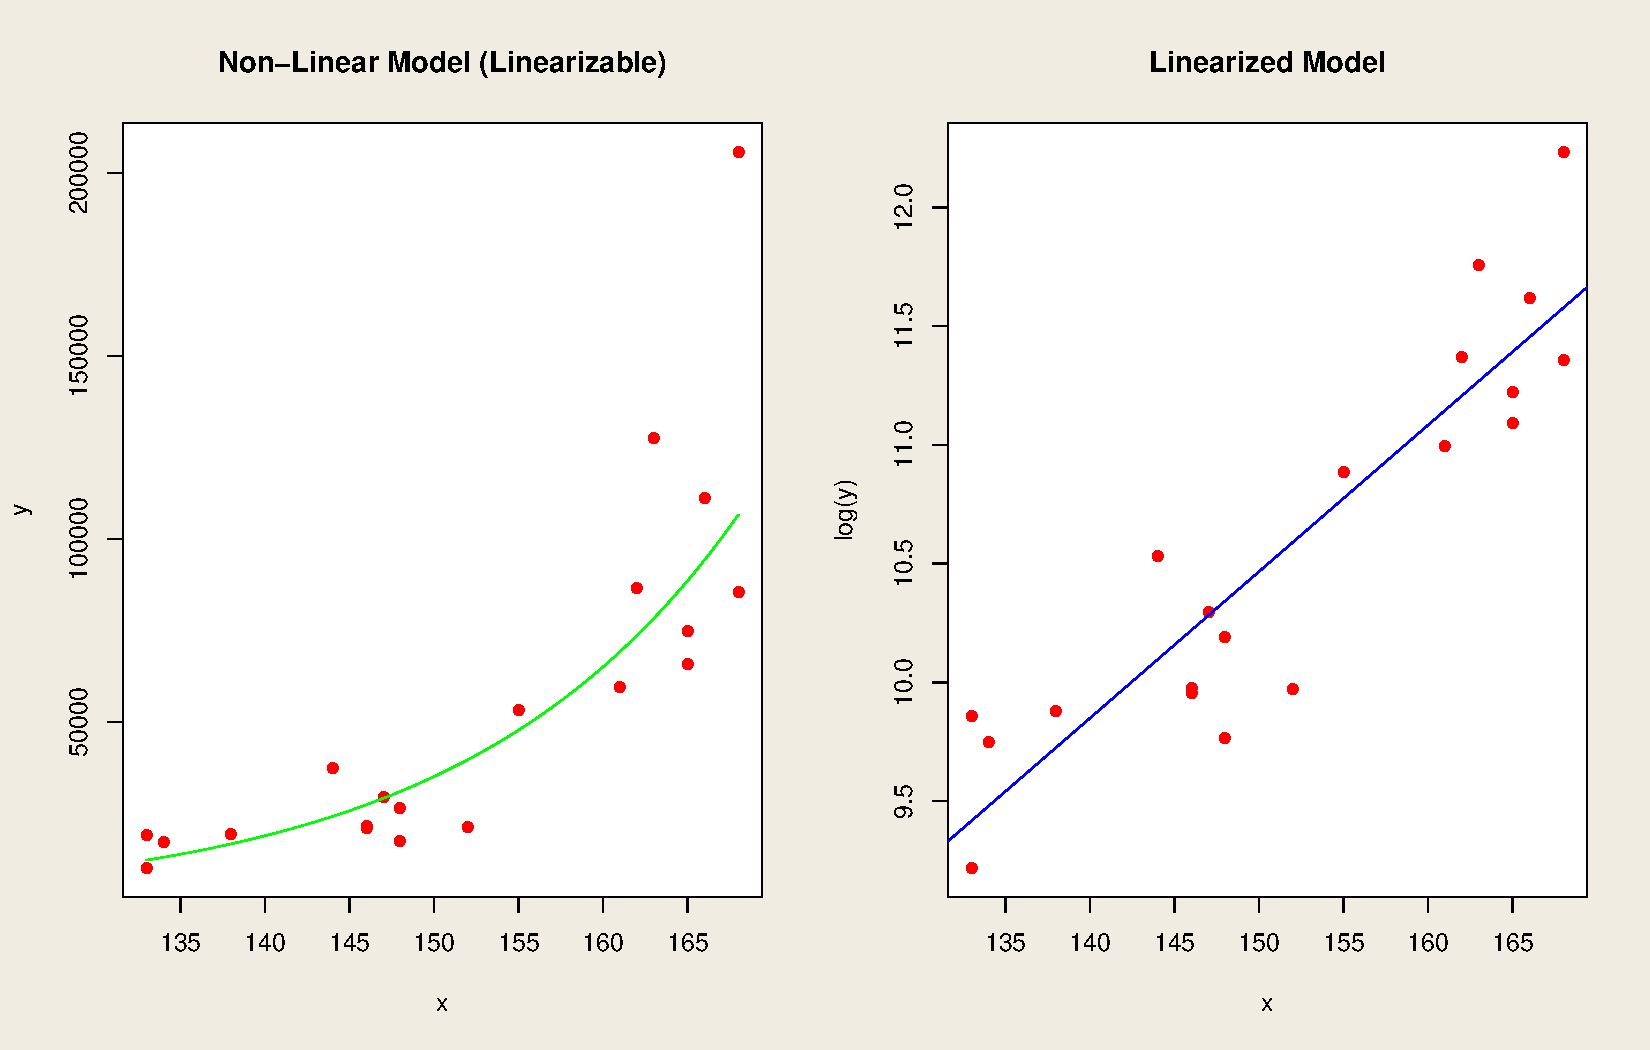
\includegraphics[scale=0.40]{6_nonlinear}
  \end{center}
\end{frame}



\livelloA{Estimation of the model}

\livelloB{Linear regression hypothesis}

\begin{frame}
  \vspace*{.25cm}
  \begin{itemize}
    \item The \textbf{main hypothesis} of the linear regression is that the structural link between the dependent variable, the explanatory variables' parameters and the error term is, as it has been expressed in the previous formula, linear. 
    \vspace*{.5cm}
    \item Futher \textbf{hypothesis} on the behavior of the \textbf{error} $ \vect{\varepsilon} $ are added to the main hypothesis. Or rather:\\
    \begin{enumerate}
     \item $ E(\varepsilon_{i}) = 0 $ \hspace{1.7cm} ($ i = 1, \dots, n $)
     \item $ \matr{X} $ not stochastic
     \item $ \varepsilon_i \sim\; N(0,\,\sigma^2_\varepsilon) $ \hspace{1cm} ($ i = 1, \dots, n $)
     \item $ Corr(\varepsilon_{i},\,\varepsilon_{i-j}) = 0 $ \hspace{0.4cm} ($ i = 1, \dots, n; 0 < j < i $)
    \end{enumerate}
  \end{itemize}
\end{frame}

\begin{frame}
  \vspace*{.5cm}
  \begin{itemize}
    \item The first hypothesis, {\boldmath$E(\varepsilon_{i})=0$}, indicates the \textbf{not systematicity of the errors}. To accept this hypothesis means to affirm that the model does not systematically ``make mistakes'' in excess or in fault compared to the central trend of the phenomenon.
    \vspace*{.5cm}
    \item The second hypothesis affirms that \textbf{the matrix} $ \matr{X} $ \textbf{is not stochastic}, or rather that the independent variables are ``firmly'' determined by the experimenter. The independent variables are not affected by gathering error; if this is present, it has to be considered unimportant. 
  \end{itemize}
\end{frame}

\begin{frame}
  \vspace*{.5cm}
  \begin{itemize}
  \item The third hypothesis, {\boldmath $ \varepsilon_i \sim\; N(0,\,\sigma^2_\varepsilon) $}, beyond restating the first one, affirms that the \textbf{errors distribution has to be gaussian}, and \textbf{the errors variability has to be constant}. This means that the dispersion of the prediction error is not influenced, in a systematical way, by the value of the response variable or by the value of the explanatory variables. \\ To accept that the error term follows a \textbf{normal distribution}, with null mean and constant variance, allows:
  \begin{itemize}
    \item the development of hypothesis tests on the parameters (t test);
    \item the development of hypothesis tests on the whole model;
    \item a criterion for the identification of the outlier values, or rather of those observation that present an excessive gap compared to the values that have been anticipated by the model.
  \end{itemize}
  \vspace*{.25cm}
  \end{itemize}
\end{frame}

\begin{frame}
  \vspace*{.25cm}
  \begin{itemize}
    \item The fourth hypothesis, {\boldmath $ Corr(\varepsilon_{i},\,\varepsilon_{i-j}) = 0 $}, affirms that \textbf{the prediction errors are not correlated in sequence}. To accept this hypothesis means being able to affirm that the time order of the observations collection does not affect the behavior of the response variable. 
    \item The four previous statements represent the hypothesis that undergo the gaussian linear model. 
    \item If the empirical data do not confirm these hypothesis, it is possible that the model is bad specified in the hypothesized functional relation and / or in the missing consideration of an important explanatory variable.
    \item The \textbf{error normality test} is one of the main point of the model's validation phase. The \textbf{graphical analysis} of the residuals and the \textbf{Anderson-Darling test} are commonly used to check this hypothesis.
  \end{itemize}
\end{frame}

\livelloB{Characteristics of estimators}

\begin{frame}
  \vspace*{.25cm}
  \begin{itemize}
    \item In the previous slides we showed how it is possible to calculate the coefficients estimations  $ \vect{\beta} $ towards the ordinary least squares method. The values $ \vect{\hat{\beta}} $ represent the \textbf{estimates} of $ \vect{\beta} $.
    \vspace*{.25cm}
    \item Each observations is given by the sum of a \textbf{structural componenent} (or deterministic one) and by an \textbf{aleatory element} {$ \varepsilon_i $}. As consequence, the sample of values $ \vect{y} $ that has been collected, with the same values of the matrix $ \matr{X} $, represents one, among the infinite samples, of the realizations of the random $ \varepsilon_i $.
    \vspace*{.25cm}
    \item The vector $ \vect{\hat{\beta}} $ results then a \textbf{random variable} with a specific distribution, which can be calculated in the linear regression.
  \end{itemize}
\end{frame}

\begin{frame}
  \vspace*{.25cm}
  \begin{itemize}
    \item If the five statements of the gaussian linear model are valid, it can be demonstrated that:
    \begin{itemize}
      \item $ E(\vect{\hat{\beta}}) = \vect{\beta} $, or rather that $ \vect{\hat{\beta}} $ is one \textbf{not distorted estimator} of the parameters vector $ \vect{\beta} $;
      \item $ Var(\hat{\beta_{j}}) = \sigma^2_{\varepsilon} \cdot g_j(\matr{X})$, where $\sigma^2_{\varepsilon}$ is the error variance $\varepsilon$  $g_j(\cdot)$ is a function (that can be calculated, deterministic and different for each $ j $) of the data  $ \matr{X} $ and, in particular, of the number $ n $ of sample observations: $ g_j(\matr{X})$ tends to decrease when $n $ increases.
    \end{itemize}
    \vspace*{.25cm}
    \item It can be demonstrated that { $\vect{\hat{\beta}} $ } is an \textbf{efficient estimator}, or rather with the smallest variance among the estimators of the same parameter, and it is with mean null error.
    \vspace*{.25cm}
    \item Furthermore, if the distributive normality of $ \vect{\varepsilon} $ is valid, it is possible to demonstrate that also the single estimated parameters ($ \hat{\beta}_j $) follow a normal distribution. 
  \end{itemize}
\end{frame}

\livelloB{Estimation of the variance estimations}

\begin{frame}
  \vspace*{.25cm}
  \begin{itemize}
    \item If it wants to be estimated the variance estimations ($ Var(\hat{\beta_{j}}) $), the result has to be an estimation $ \hat{\sigma}^2_{\varepsilon} $ of $ \sigma^2_{\varepsilon} $.
    \vspace{1cm} \item The term $ \hat{\sigma}^2_{\varepsilon} $ represents the \textbf{estimated standard deviation} of the prediction error. The standard deviation of the prediction error is the residual variability for the dependent variable $ \vect{y} $, once that the variability due to the ``predictable'' or deterministic element $ f(\cdot) $ of the model has been removed. $\hat{\sigma}^2_{\varepsilon}$ is calculable as the square of:
      $$ \hat{\sigma}_{\varepsilon} = \sqrt{\frac{\sum_{i=1}^n{\left[ y_i-f\left( \vect{x_i}; \vect{\beta} \right)  \right] ^2 }} {n-p-1}} $$
  \end{itemize}
\end{frame}

\livelloB{An example of parameters estimation}

\begin{frame}
  \begin{itemize}
    \item In the slides about the simple linear regression it has been presented an example of parameters estimation with the ordinary least squares method.
    \item Another example of estimation is presented afterwards. The plot shows the relation between a variable $ x $ and a variable $ y $.
  \end{itemize}
  \begin{center}
    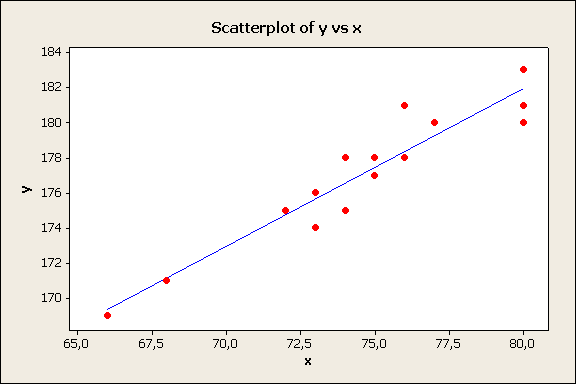
\includegraphics[scale=0.45]{6_18.png}
  \end{center}
\end{frame}

\begin{frame}
  \vspace*{.25cm}  
  \begin{itemize}
    \item The relation between $ y $ and $ x $ has been modeled with a simple linear regression.
    \item The estimated \textbf{coefficients} of the regression line, reported above, are $y=109.95 + 0.90 \cdot x$
    \item The coefficient 0.90 is the \textbf{slope}. It indicated the (mean) increase of the dependent variable if $x$ increases one unity.
    \item The value 109.95 represents the \textbf{intercept} of the line. It indicates which is the mean value of  $y$ if $x$ is (hypothetically) equal to 0. The pratic interpretation of the intercept depends on the sense the null value in all the explanatory variables has on the application taken into consideration.
   \item  The value of $ \hat{\sigma}^2_{\varepsilon} $ estimated for this model is equal to 1.244. This value represents the estimation of the \textbf{residual variance} of the y, after the link between the y and the x.
  \end{itemize}
\end{frame}



\livelloA{Validation of the model}

\livelloB{Decomposition of the variability}

\begin{frame}
  \begin{itemize}
    \item The \textbf{excellence of a regression model} as regards its adaptation to the data depends on the variability quota of the dependent variable that the model is able to explain.
    \item If the intercept is included in the regression function, the \textbf{total deviance} of the dependent variable (\textbf{SST}) can be decomposed in the sum of two elements, \textbf{SSR} and \textbf{SSE}:
  \end{itemize}
  \begin{align*}
    \text{SST} &= \sum_{i=1}^n {(y_i - \overline{y})^2} \\
    \text{SST} &= \text{SSR} + \text{SSE} \\
    \text{SSR} &= \sum_{i=1}^n {\bigl(y_i-f( \vect{x_i}; \vect{\beta} ) \bigr)^2} \\
    \text{SSE} &= \sum_{i=1}^n {\bigl(f( \vect{x_i}; \vect{\beta} ) - \overline{y} \bigr)^2} \\
  \end{align*}
\end{frame}

\begin{frame}
  \vspace*{.25cm}
  \begin{itemize}
    \item \textbf{SST}: \textit{Sum of Squares of Total} 
    \item \textbf{SSE}: \textit{Sum of Squares Explained} 
    \item \textbf{SSR}: \textit{Sum of Squares of Residuals} 
    \vspace*{.5cm}
    \item In other words, the whole variability of the phenomenon we are studying (SST) can be divided into two elements: the ``explained'' element of the regression (SSE) and the ``residual'' element (SSR).
    \vspace*{.5cm}
    \item Towards the sum of squares of the differences between the expected values and the mean, \textbf{SSE} measures the variabilty quota that the model catched. 
    \item Towards the sum of squares of the differences between the expected values and the observed ones, \textbf{SSR} measures the variability side of the y that the regression model did not catch.
  \end{itemize}
\end{frame}

\livelloB{Decomposition of the variability - coefficient of determination}

\begin{frame}
  \vspace*{.5cm}
  \begin{itemize}
    \item Thence, a whole excellence index of the model is given by the weight of SSE on SST. The greater is the quota of SSE on SST, the greater is the percentage of variability of the y explained by the regression model.
    \vspace*{.75cm}
    \item The adaptation index that sums up the relation between the elements of the variance is the \textbf{coefficient of determination}:
      \vspace*{.4cm} $$ R^2 = \frac{SSE}{SST} = 1 - \frac{SSR}{SST} $$
  \end{itemize}
\end{frame}

\begin{frame}
  \vspace*{.25cm}
  \begin{small}
    \begin{itemize}
      \item $ R^{2} $ (R-squared) is an index that is always included between 0 and 1, included;
      \item $ R^{2} $ is, at the maximum, equal to one when all the variability is explained by the regression function (or rather, when the regression function ``crosses'' all the points);
      \item $ R^{2} $ is, at the minimum, equal to zero when the regression function is not more useful than the sample mean in order to describe the phenomenon;
      \item $ R^{2} $ assumes intermediate values in function of the ``adaptation level'' (or rather of the ability to explain the phenomenon) of the regression function.
      \item The $ R^{2} $  values is decreasing with the number of explanatory variables introduced in the regression function. This means that it is possible to obtain a $R^{2}$ value really near to 1 simply adding explanatory variables even though they are not really ``linked'' with the analysed phenomenon.
    \end{itemize}
  \end{small}
\end{frame}

\begin{frame}
  \begin{itemize}
    \item The value of the coefficient of determination does not depend on the ``direction'' of the estimated relation between independent variables and the dependent variable. Or rather, the value of the coefficient of determinaton does not depend on the ``sign'' of the estimated parameters but by the residual variability degree for the y that results from leaving the ``captured'' variability from the estimated model.
    \item To raise the adaptation index does not have to overlook the analytic parsimony and the simplicity of the interpretation. In general words, it is preferable to have values of the $R^{2}$ coefficient slightly lesser if the model that results is more easily interpretable;
    \item In general, a $ R^{2} $ value can be defined as good if it has been compared to the $ R^{2} $ value of alternative models for the same phenomenon.
  \end{itemize}
\end{frame}

\begin{frame}
  \vspace{-0.2cm}
  \begin{center}
    \ifthenelse{\equal{\materiale}{jmp}}
      {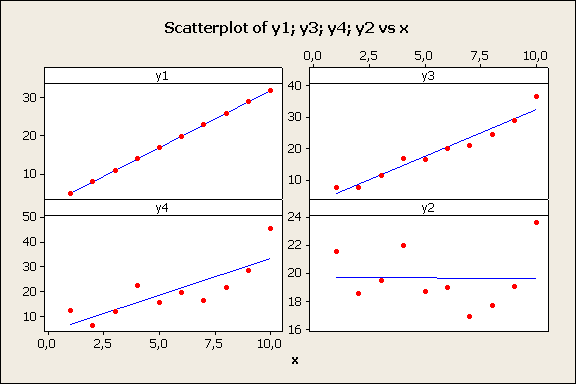
\includegraphics[scale=0.38]{6_25.png}}
      {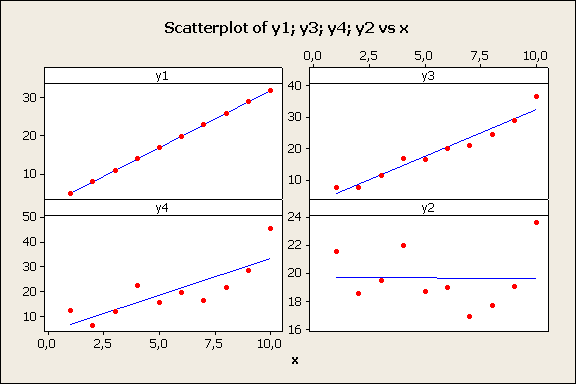
\includegraphics[scale=0.5]{6_25.png}}  
  \end{center}
  \vspace{-0.2cm}
  These plots represent linear relations between the y and the x with decreasing $ R^{2} $ values. The panel in the top left-hand corner shows a model with $ R^{2} = 1 $. The panel in the low right-hand corner shows the model with $ R^{2} = 0 $.
\end{frame}

\begin{frame}
  \vspace*{.25cm}
  \begin{itemize}
    \item As the $R^{2}$ value is also influenced by the presence of explanatory variables, even though these are not effectively linked to the analysed phenomenon, it has been considered the possibility to introduce a variation of the index, the \textbf{adjusted} {\boldmath$R^{2}$}:
      $$\overline{R}^{2}=1-\frac{(n-1)}{(n-p-1)}\frac{SSR}{SST}=1-\frac{(n-1)}{(n-p-1)}(1-R^2)$$
    \item The adjusted $R^{2}$ has the following \textbf{characteristics}:
    \begin{itemize}
      \item The adjusted $R^{2}$ is lesser or equal to 1, but can be also lesser than 0;
      \item The \textbf{correction factor} $-\frac{(n-1)}{(n-p-1)}$ ``reduces'' the $R^{2}$ value of an element that depends on the \textbf{number of explanatory variables} that have been used. The most are the explanatory variables, the most the adjusted $R^{2}$ will be lesser than the $R^{2}$.
    \end{itemize}
  \end{itemize}
\end{frame}

\livelloB{The hypothesis test}

\begin{frame}
  \vspace*{.25cm}
  \begin{itemize}
    \item With the formula we presented, it is possible to obtain the curve coefficients that is better adapted to the noticed data, with any dispersion points shape.  
    \item Anyway, the \textbf{curve coefficients calculation} is not enough for the statistician. It would be possible to have:
    \begin{itemize}
      \item a \textbf{significative relation} (or ``real'') between the independent variables and the explanatory one, if the point dispersion around the curve is small;
      \item a \textbf{not significative relation} (or random), when the dispersion points around the curve is almost equal to the one around the mean.
    \end{itemize}
    \item The \textbf{hypothesis test} allows to verify in which of the two conditions we are working. It is possible thanks to the assumptions that have been made on the errors distribution. 
  \end{itemize}
\end{frame}

\begin{frame}
  The \textbf{hypothesis test} on the linear regression model can be:
  \begin{itemize}
    \item Hypothesis test \textbf{on the coefficient linked to a single explanatory variable}. With this test it is possible to check the hypothesis that the coefficient of the variable taken into consideration can be considered statistically equal to a specific value. For this kind of hypothesis test, the error normality allows the use of the \textbf{Student's t} distribution.
    \item Nullity hypothesis test of \textbf{more than one explanatory variable coefficient} (possibly on all of them). The error normality allows the use of the \textbf{F of Fisher-Snedecor} distribution.
    \item Testing \textbf{on the assumptions of the gaussian linear model}. There are tests to check: normality of errors, the independence of errors,  the constant variability of the errors (homoscedasticity).
  \end{itemize}
\end{frame}

\livelloB{Hypothesis test on a coefficient}

\begin{frame}
  \vspace*{.05cm}
  \begin{itemize}
    \item The aim of the \textbf{hypothesis test on a coefficient} is to check the \textbf{hyphotesis} that the ``true'' value of a parameter $ \beta_j $ is \textbf{equal to an hypothesized value} $ \beta_{H_0} $, against the hypothesis that this \textbf{different} from $ \beta_{H_0} $.
    \item Setting up $ \beta_{H_0} = 0 $, it is verified if the estimated effect on the sample for the analysed parameter is  ``real'' and ``concrete'' for the whole population (I accept $ \beta_{H_0} \neq 0 $), or it is due to random fluctuations in the analysed sample (I accept $ \beta_{H_0} = 0 $). This is the \textbf{statistical significativity test} of a coefficient.
    \item If we want to formulate an hypothesis test in a formal way, the hypothesis (called \textbf{null hypothesis}) is\\
    \vspace*{.15cm}
    \hspace*{1cm}$H_0:\,\beta_{j} = \beta_{H_0}$\\
    \vspace*{.15cm}
    against the \textbf{alternative hypothesis}\\
    \vspace*{.15cm}
    \hspace*{1cm}$H_{A}:\, \beta_{j}\neq \beta_{H_0}$
  \end{itemize}
\end{frame}

\begin{frame}
  The statistical hypothesis testing about a parameter is based on the following statistical basis, that can be demonstrated:
  \vspace*{-.15cm}
  \begin{itemize}
    \item If $ H_0 $ is true, and $ \sigma_\varepsilon $ is known, then the \textbf{standard coefficient {\boldmath $ \hat{\beta}_j $}} follows a standard normal distribution:
      $$ \frac{\hat{\beta}_j-\beta_{H_0}}{\sigma_{\varepsilon}\sqrt{g_j(X)}}\sim\;N(0,\,1) $$
    \item As the \textbf{standard deviation} of the regression error \textbf{is not known} and has to be estimated from the data, the used index is the following one:
      $$ t = \frac{\hat{\beta}_j-\beta_{H_0}}{\hat{\sigma}_{\varepsilon}\sqrt{g_j(X)}} $$
    \item With $ H_0 $, the index $ t$ follows a \textbf{Student's t} distribution with $ (n-(p+1)) $ degrees of freedom, where $ p + 1 $ is equal to the number of estimated parameters.
  \end{itemize}
\end{frame}

\begin{frame}
  \vspace*{.75cm}
  \begin{itemize}
    \item The $ H_0 $ ``null'' hypothesis is accepted if $ \abs{t} $ is ``small'', and therefore, if the difference $ \abs{\hat{\beta}_j-\beta_{H_0}} $ is ``small'' compared to the standard error of $ \hat{\beta} $.
    \vspace*{.75cm}
    \item Affirming that a regression coefficients is different from the $ \beta_{H_0}  $  hypothesize value means that $ \hat{\beta}_j $ has an ``high'' distance from $ \beta_{H_0} $ compared to its standard error, measured by the element in the denominator $\hat{\sigma}_{\varepsilon}\sqrt{g_j(X)}$.
  \end{itemize}
\end{frame}

\begin{frame}
  \vspace*{.75cm}
  \begin{itemize}   
    \item When significativity of the coefficient $ \beta_j $ is verified, it is check if the $j$th explanatory variable does not influence the dependent variable, and then if the  $ \beta_j $ value can be null ($ \beta_{H_0} = 0 $).
    \vspace*{.75cm}
    \item The significativity of the coefficient $ \beta_j $ is confirmed if:
      $$ \abs{t} = \frac{\mid\hat{\beta}_j\mid }{\hat{\sigma}_{\varepsilon}\sqrt{g_j(X)}} > t_{n-p-1,\,\frac{\alpha}{2}} $$
      or rather if the absolute value of the $ t $ statistics is greater than the tabulated value of the t of Student's distribution with $ n-p-1 $ degrees of freedom for the significativity level that has been required ($ \alpha $).
  \end{itemize}
\end{frame}

\begin{frame}
  \vspace*{.5cm}
  \begin{itemize}
  \item As the distributive family $\hat{\beta}_j$ is the Student's t, some confidance intervals for the parameter  $\beta_j$ can be easily obtained if it is based on the distribution characteristics themselves. 
  \vspace*{.5cm}
  \item The confidence interval with interval $1-\alpha$ for the parameter $\beta_j$ is expressed by:
    $$\hat{\beta}_j-t_{n-p-1;\,\frac{\alpha}{2}}\cdot \widehat{if(\hat{\beta}_j)}\leqslant\beta_j\leqslant\hat{\beta}_j+t_{n-p-1;\,\frac{\alpha}{2}}\cdot \widehat{if(\hat{\beta}_j)}$$
    where $\widehat{se(\hat{\beta}_j)}=\hat{\sigma}_{\varepsilon}\sqrt{g_j(X)}$
\end{itemize}
\end{frame}

\livelloB{The hypothesis test on more than one coefficient}

\begin{frame}
  \vspace{-0.10cm}
  \begin{itemize}
    \item Another possible hypothesis test on the gaussian linear model is the \textbf{test on the simultaneous nullity of more coefficients} linked to specific variables. 
    \item This statement can be expressed, without loosing the generality, like $H_0:\beta_{p-J}=\cdots=\beta_p=0$, where $J$ is the number of null parameters. The alternative hypothesis will state that at least a $\beta_j$ ($p-J\leqslant j\leqslant p$) is different from.
    \item The \textbf{uses} of this kind of hypothesis test can be:
    \begin{itemize}
      \item to verify if an alternative regression model, with a smaller number of explanatory variables, has the same predictive ability than the most complex model, in favor of the interpretative parsimony;
      \item to verify if \textbf{the model that has been realised explains the phenomenon better than the sample mean} of the dependent variable, or rather to verify if the developed model is better than  regression model where all the coefficients linked to the explanatory variables are null.
    \end{itemize}
  \end{itemize}
\end{frame}

\begin{frame}
  \vspace*{.25cm}
  \begin{itemize}
    \item $ S_{0} $ is the \textbf{residuals deviance} of regression of the estimated model with the hypothesize \textbf{null} \textbf{coefficients} of the $ J $ chosen variabiles.
    \vspace*{.25cm}
    \item $ S_{1} $ is the residuals deviance of regression of \textbf{complete estimated model}, then, with the hypothesis $ H_0 $ that all the hypothesized coefficients are null.
    \vspace*{.25cm}
    \item Then, with the $ H_0 $ null hypothesis, the ratio $ {(S_0-S_1)}/{\sigma^2_{\varepsilon}} $ follows a $ \chi^2_{J} $ distribution.
    \vspace*{.25cm}
    \item It is possible to demostrate that, with the $ H_0 $ hypothesis, the ratio 
      $$ F = \frac{S_0-S_1}{J}/{\frac{S_1}{n-p-1}} \sim F_{J, (n-p-1)} $$ \\
  \end{itemize}
\end{frame}

\begin{frame}
  \vspace*{.75cm}
  \begin{itemize}
    \item The nullity hypothesis of the $ J $ coefficients is ``translated'' in statistical words with the hypothesis that \textbf{the ratio {\boldmath $ F $} is ``small''}. 
    \vspace*{.75cm}
    \item This ratio, with $ H_0 $, is distributed like a F of Fisher-Snedecor with parameters $ J, (n-p-1) $. The null hypothesis will be refused if the $ F $ ratio exceedes the critical value, or rather if:
      $$ F > F_{J,\,n-p-1;\,1-\alpha} $$
  \end{itemize}
\end{frame}

\begin{frame}
  \vspace*{.5cm}
  \begin{itemize}
    \item If the hypothesis test regards the coefficient significativity linked to \textbf{all} the explanatory variables that gave been used, the $ J $ parameter has to be replaced with $ p $.
    \vspace*{.25cm}
    \item In conclusion, if the hypothesis test regards a \textbf{single parameter}, it is demonstrated that the F test is equal to the \textbf{t test}.
    \vspace*{.25cm}
    \item The \textbf{F test} is used for \textbf{automatic selection method for the explanatory variables} (\textbf{stepwise} regression algorithm). These algorithms add and remove variables comparing alternative models (with diffent variables included) according to the F test values.
  \end{itemize}
\end{frame}

\livelloB{Testing the assumption of the gaussian linear model}

\begin{frame}
  \vspace*{.25cm}
  \begin{itemize}
    \item The last step, fundamental, of the regression analysis is \textbf{testing the assumption of the gaussian linear model}. This test is done studying the residuals with graphic tools and eventually with statistical tests.
    \vspace*{.25cm}
    \item The \textbf{residuals analysis} allows to verify the main assumptions for the applicability of the regression techniques:
    \begin{normalsize}
      \begin{itemize}
        \item \textbf{gaussianity} of the residuals;
        \item \textbf{independence} of the residuals;
        \item \textbf{homoscedasticity} (uniform variance) of the residuals.
      \end{itemize}
    \end{normalsize}
    \vspace*{.25cm}
    \item Beyond these assumpotions, the residuals analysis allows to evaluate, within some limits, if the chosen model is adequate and if other explanatory variables are needed.
  \end{itemize}
\end{frame}

\begin{frame}
  \begin{itemize}
    \item As we have already shown, the \textbf{estimated residuals} {\boldmath$\hat{\varepsilon}_i$} are an estimation of the gaussian random errors ($\varepsilon_i$), and are defined like:
      \vspace{-0.3cm} $$ \hat{\varepsilon}_i = y_i-\hat{y}_i = y_i-f(\vect{x_i};\vect{\hat{\beta}}) $$
    \item For the residuals that come from \textbf{the least squares estimation}, it is always valid:
      \vspace{-0.3cm} $$ \sum_{i=1}^n \hat{\varepsilon}_i = 0 $$
    \item Beyond the residuals that have just been mentioned, there are different versions of them (\textit{deleted} residuals, Pearson residuals, \textit{studentized} residuals, Cook residuals , etc$\dots$), with different finalities that will be partially explained later.
    \item In general, in order to evaluate if the applicability hypothesis of the model are adequate, the \textbf{instruments} are mainly \textbf{graphics}. Here there are some (not exhaustive) examples.
  \end{itemize}
\end{frame}

\begin{frame}
  \vspace*{-.5cm}
  \begin{center}
    \ifthenelse{\equal{\materiale}{jmp}}
      {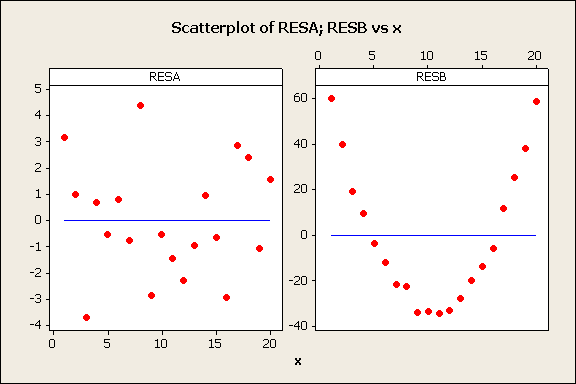
\includegraphics[scale=0.48]{6_37.png}}
      {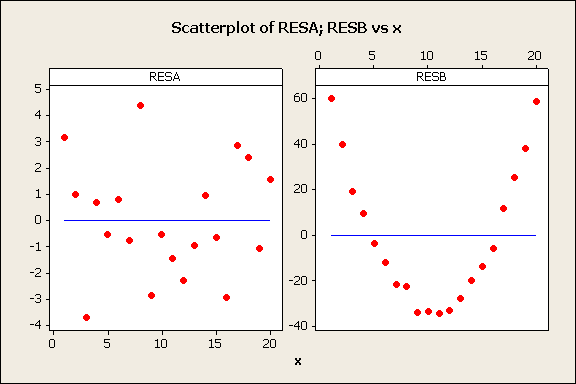
\includegraphics[scale=0.48]{6_37.png}}
  \end{center}
  \vspace*{-.3cm}
  The graphics represents two case of linear regression residuals with an explanatory variable. The panel on the left shows an ideal behavior: the residuals are placed in a random way around the null value. The other plot shows a parabolic trend: a quadratic element for the x has to be added.
\end{frame}

\begin{frame}
  \begin{center}
    \ifthenelse{\equal{\materiale}{jmp}}
      {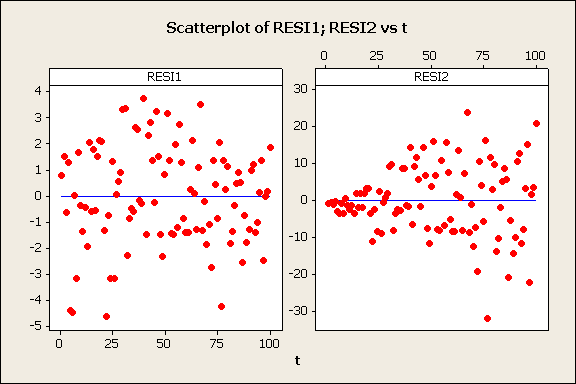
\includegraphics[scale=1.50]{6_38.png}}
      {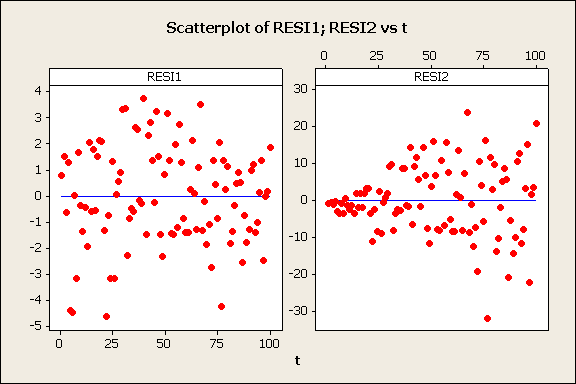
\includegraphics[scale=0.48]{6_38.png}}
  \end{center}
  The plot on the left panel shows residuals that have a constant variability compared to the appearance order. The residuals of the right panel show increasing variability compared to the appearance order.
\end{frame}

\begin{frame}
  \begin{center}
    \ifthenelse{\equal{\materiale}{jmp}}
      {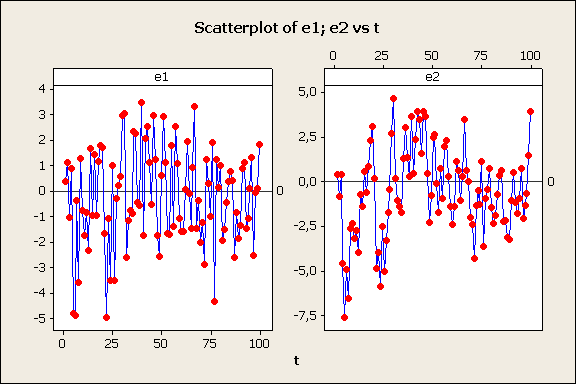
\includegraphics[scale=1.50]{6_39.png}}
      {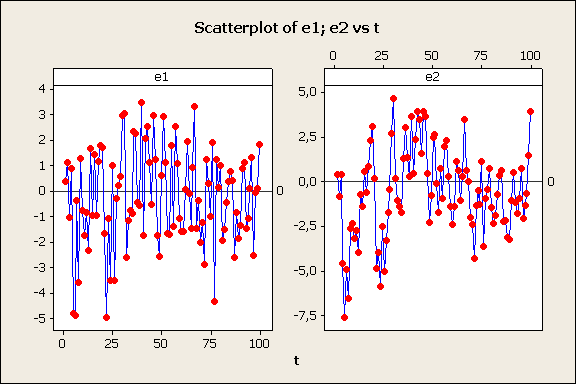
\includegraphics[scale=0.48]{6_39.png}}
  \end{center}
  The plot of the left panel shows not correlated residuals. The plot of the right panel shows residuals with autocorrelation compared to the appearance order.
\end{frame}

\begin{frame}
  \begin{center}
    \ifthenelse{\equal{\materiale}{jmp}}
      {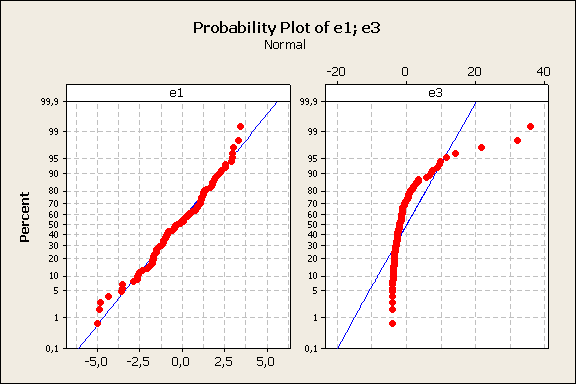
\includegraphics[scale=1.50]{6_40.png}}
      {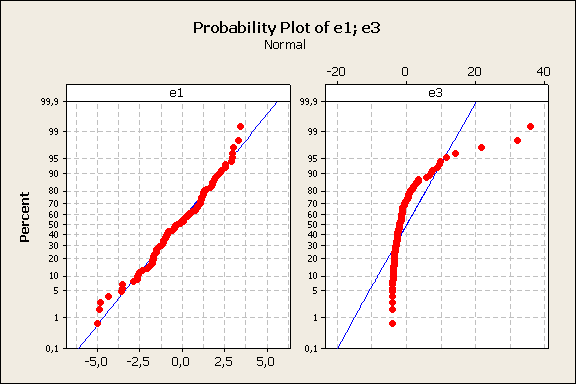
\includegraphics[scale=0.48]{6_40.png}}
  \end{center}
  The plot of the left panel shows residuals that follow a normal distribution. The residuals in the right panel cannot be considered normally distributed.
\end{frame}

\begin{frame}
  \vspace*{-.15cm}
  \begin{itemize}
    \item The \textbf{residuals plot towards the independent variables} (or prediction value) does not have to show an identifiable functional trend .
    \begin{itemize}
      \item If the residuals are vaguely placed around the zero, it means that the side of the variability that has not been catched by the linear regression is not identifiable if we specify a different functional relation between the y and the explanatory variable.
      \item If the residuals show a noticeable functional relation, it is possible that the linear model does not adequately catch the functional relation among the data.
    \end{itemize}
    \item The residuals must have constant variability (\textbf{homoscedasticity}). Or rather, the residual scatterplot compared to the values of the independent variables (or the prediction values) does not have to show an evident increase or decrease in the variability. If the homoscedasticity does not verify it can be because of:
    \begin{itemize}
      \item the missing inclusion of an important explanatory variable;
      \item the wrong specification of the functional relation among the data.
    \end{itemize}
  \end{itemize}
\end{frame}

\begin{frame}
  \vspace{.5cm}
  \begin{itemize}
    \item The residuals have to be \textbf{independent} among them, or rather they do not have to be influenced by the previous values. The presence of autocorrelation in the residuals means that there is dependence among the residuals. The \textbf{autocorrelation} of the residuals can be due to:
    \begin{itemize}
      \item a wrong specification of the functional link among the variables;
      \item not inclusion of a explanatory variable linked to the time in the model.
    \end{itemize}
  \vspace{.5cm}
  \item The residuals have to be distributed according to a \textbf{normal} law, with parameters $ N(0, \sigma_\varepsilon)$. If this assumption is verified, then the hypothesis tests on the significativity of the model parameters are verified too. 
  \end{itemize}
\end{frame}

\begin{frame}
  \vspace{.5cm}
  \begin{itemize}
    \item The residuals normality test can be done with \textbf{normal probability plot} and with \textbf{adaptation test} (e.g. \textbf{Anderson-Darling}).
    \vspace{.5cm}
    \item Of the residuals are not normally distributed, it could be appropriate to:
    \begin{itemize}
      \item specify the model, changing the functional shape and/or the explanatory variables;
      \item use more complex regression models (ex. GLM).
    \end{itemize}
  \end{itemize}
\end{frame}

\livelloB{Test of influent points}

\begin{frame}
 \begin{itemize}
    \item Other diagnostic instruments to verify the model are the ``leverage points'' or ``influent points''.
    \item Please observe the following plot.
  \end{itemize}
  \begin{center}
    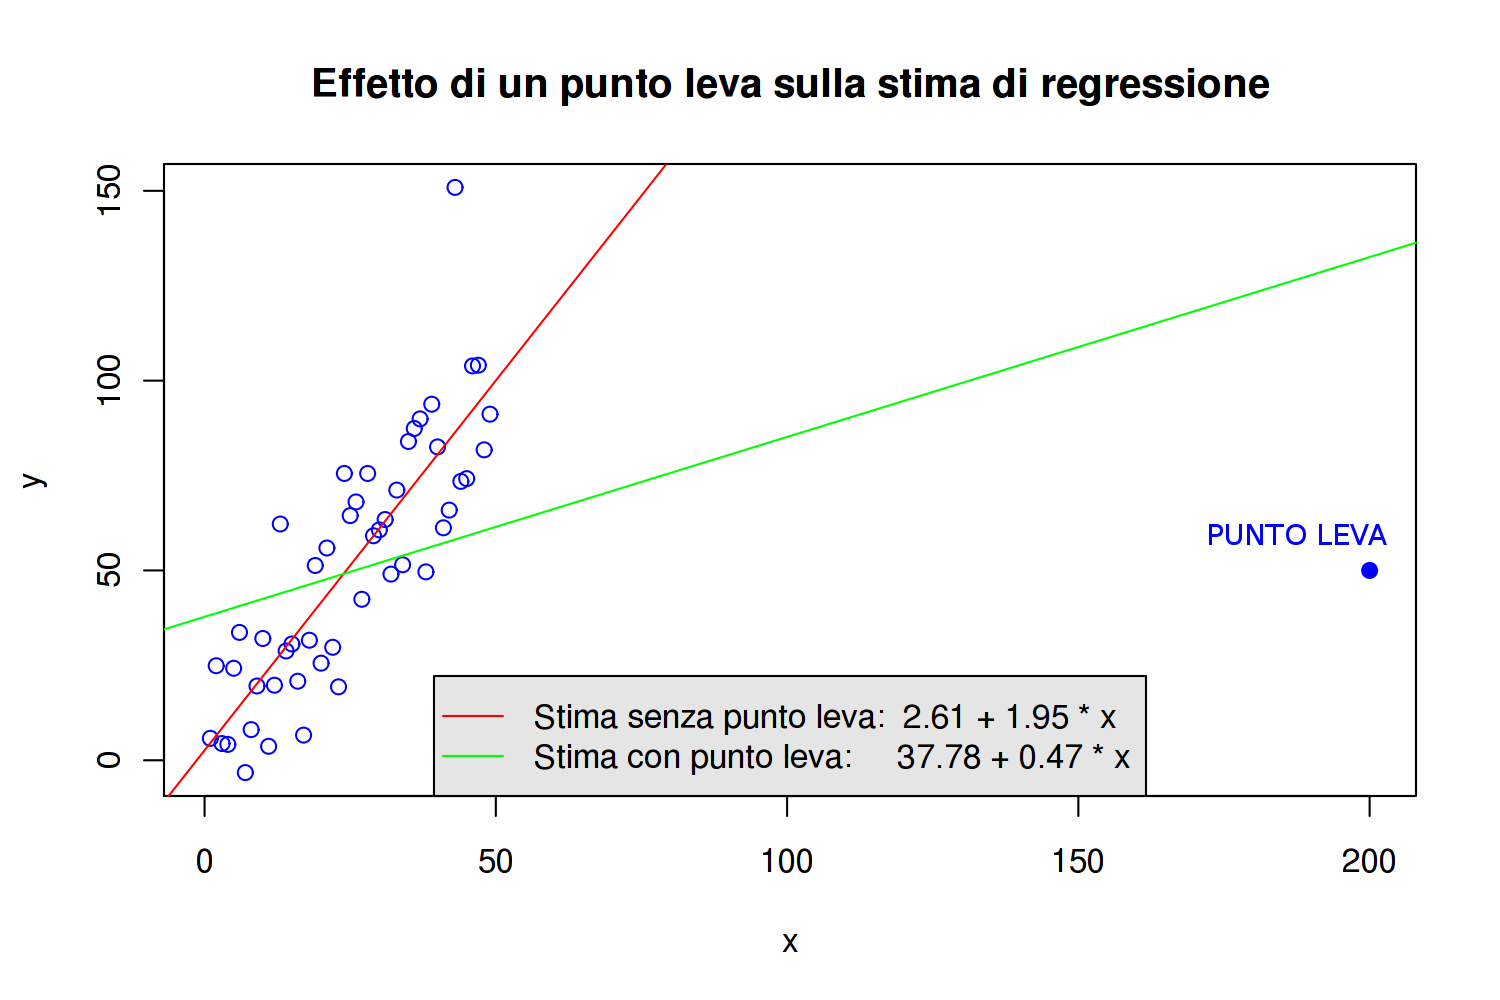
\includegraphics[scale=0.48]{6_regrPuntoLeva.png}
  \end{center}
\end{frame}

\begin{frame}
\vspace{0.5cm}
  \begin{itemize}
    \item In the previous plot 50 points have been drawn. One of them (highlighted with the ``full'' point) is an ``outlier'', in the sense that it is really far from the others.
    \vspace{0.5cm}
    \item The two regression lines have been estimated excluding (the red line) and including (the green line) the ``outlier'' point.
    \vspace{0.5cm}
    \item The outlier point clearly ``pushes down'' the estimated regression line, modifying the parameters estimations.
  \end{itemize}
\end{frame}

\begin{frame}
\vspace{0.5cm}
  \begin{itemize}
    \item When a point (usually outlier) influences on the parameters estimation, then it is called \textbf{leverage point}.
    \vspace{0.5cm}
    \item The leverage points come from the fact that the least squares techniques look for the curve that minimizes the \textbf{square} difference between the observed values and the estimated values of the curve itself.
    \vspace{0.5cm}
    \item Not all of the outlier point are leverage points too.
  \end{itemize}
\end{frame}

\begin{frame}
  \begin{itemize}
    \item In order to identify the influent points, beyond the plots, two kinds of indicators can be used:
    \begin{itemize}
      \item the \textbf{leverage} values;
      \item the \textbf{Cook's distances}.
    \end{itemize}
    \vspace{0.75cm}
    \item The formula for both the indexes are quite complex. 
  \end{itemize}
\end{frame}

\begin{frame}
  \begin{itemize}
    \item The leverage value for the $i$th ($i=1, \dots, n$) observation comes from the $i$th value of the diagonal of the (\textit{hat matrix}): $\matr{X}(\matr{X}^T\matr{X})^{-1}\matr{X}^T$.
    \vspace{0.5cm}
    \item The Cook's distance for the $i$th observation is proportional to 
      $$ r_i = \sum_{k=1}^n (\hat{y}_k - \hat{y}_{k,(i)})^2 $$
      where $ \hat{y}_k $ is the least squares estimation of the $ k $th observation of the y. $ \hat{y}_{k,(i)}$ represents the least squares estimation of the $ k $th observation of the y obtained by removing the $ i $th observation.
  \end{itemize}
\end{frame}

\begin{frame}
  \begin{itemize}
    \item For both the indicators, a great value represents the potential possibility that the point taken into consideration is a leverage point. This is not sure for the leverage points.
    \item In the case of the example, the leverage point obtains a \textit{hat} (leverage) value equal to 0.7588, while all the other points obtain a value not greater than 0.04.
    \item The Cook's distance value, for the leverage point is equal to 48.83, while all the other points obtain a value not greater than 0.15.
    \item In order to define a threshold in which it is possible to establish if a point is or not a leverage point, with the Cook's distance it is possible to use the distribuition $ F_{2,n-2} $ as reference point. 
    \item Alternatively, for the Cook's distance is usually considered ``great'' a value which is greater than 1.
\end{itemize}
\end{frame}



\livelloA{Use of the model}

\livelloB{The prediction}

\begin{frame}
  \vspace*{.25cm}
  \begin{itemize}
    \item Towards the \textbf{prediction}, the developed and tested model can be used to predict \textbf{values of the dependent variable} (the y) for values of the \textbf{x} even though they have not been found in the experimental phase.
    \vspace*{.5cm}
    \item The following statements are valid:
    \begin{itemize}
      \item under the statistical point of view, every prediction or estimation of the y is valid only within the \textbf{experimental variation field} of the independent variable (the x);
      \vspace*{.15cm}
      \item in the linear regression, the regression model (or, to better say, the function) does not often correspond to the real mathematical relation that exist between the independent variables and the dependent variable.
    \end{itemize}
  \end{itemize}
\end{frame}

\begin{frame}
  \vspace*{.5cm}
  \begin{itemize}
    \item Most of the times, the chosen \textbf{model} represents \textbf{an approximation of the existing relation}. Furthermore, it is known that with a quite complex function, it is always possible to describe the phenomenon.
    \vspace*{.5cm}
    \item \textbf{Extrapolating} the data out of the real observational field is an error of statistics technique. It can be accepted only in the specific context, if it is justifiable by a better knowledge of the phenomenon.
  \end{itemize}
\end{frame}

\livelloB{Confidence bands for the regression}

\begin{frame}
  \vspace*{.25cm}
  \begin{itemize}
    \item When a regression is estimated, given the experimental observations, the puntual estimations of the parameters represent the ``best value''. 
    \item Anyway, as we saw before, the parameters estimations can change within a certain range, which usually depends on the size of the standard error of estimation (take a look to the slides about the confidence intervals of the parameters).
    \item The estimation of the regression curve, can change within a certain (confidence) band.
    \item When the $\alpha$ value (usually equal to 0.05) has been chosen, it is possible to estimate the confidence bands for the regression curve.
    \item In those bands, we expected that the real regression curve ``is present'' with a confidence level equal to $(1-\alpha)$ .
  \end{itemize}
\end{frame}

\begin{frame}
  \vspace*{.25cm}
  \begin{itemize}
    \item With the``synthetic'' mathematical form (matrix), it is possible to demonstrate that the limits of the confidence intervals with level $(1-\alpha)$ for the regression curve, for a vector of explanatory (independent) variables values $\underline{x}_*$, are: \\
      \vspace*{.1cm}
      LCL: $f(\underline{x}_*;\hat{\underline{\beta}})-t_{n-p-1;\,\frac{\alpha}{2}}\cdot \sqrt{\underline{x}_*^T(X^TX)^{-1}\underline{x}_*}\cdot \hat{\sigma_\varepsilon}$ \\
      \vspace*{.1cm}
      UCL: $f(\underline{x}_*;\hat{\underline{\beta}})+t_{n-p-1;\,\frac{\alpha}{2}}\cdot \sqrt{\underline{x}_*^T(X^TX)^{-1}\underline{x}_*}\cdot \hat{\sigma_\varepsilon}$ \\
      \vspace*{.1cm}
      where $\hat{\underline{\beta}}$ is the vector of the least squares parameters estimation and the operator $^T$ represents the matrix transposition.
    \vspace{0.5cm}
    \item The size of this interval is, then, equal to $2\cdot t_{n-p-1;\,\frac{\alpha}{2}}\cdot \sqrt{\underline{x}_*^T(X^TX)^{-1}\underline{x}_*}\cdot \hat{\sigma_\varepsilon}$
  \end{itemize}
\end{frame}

\begin{frame}
  \vspace*{.25cm}
  \begin{itemize}
    \item This size \textbf{increases} in a not linear way when the distance of the vector $\underline{x}_*$ from the vector of the mean values of the columns of the matrix $X$.
    \vspace*{.25cm}
    \item The size, \textbf{decreases} in a not linear way when the numerosity of the sample, from which the estimations of $\underline{\beta}$ are obtained, increases.
    \vspace*{.25cm}
    \item The following plot shows two regression lines with confidence band at 95\%, with different sample numerosity. It has to be noticed how the bands ``broaden'' when they go away from the mean value of the independent variable, and how they ``narrow'' when the sample numerosity increases.
  \end{itemize}
\end{frame}

\begin{frame}
  \begin{center}
    \ifthenelse{\equal{\materiale}{jmp}}
    {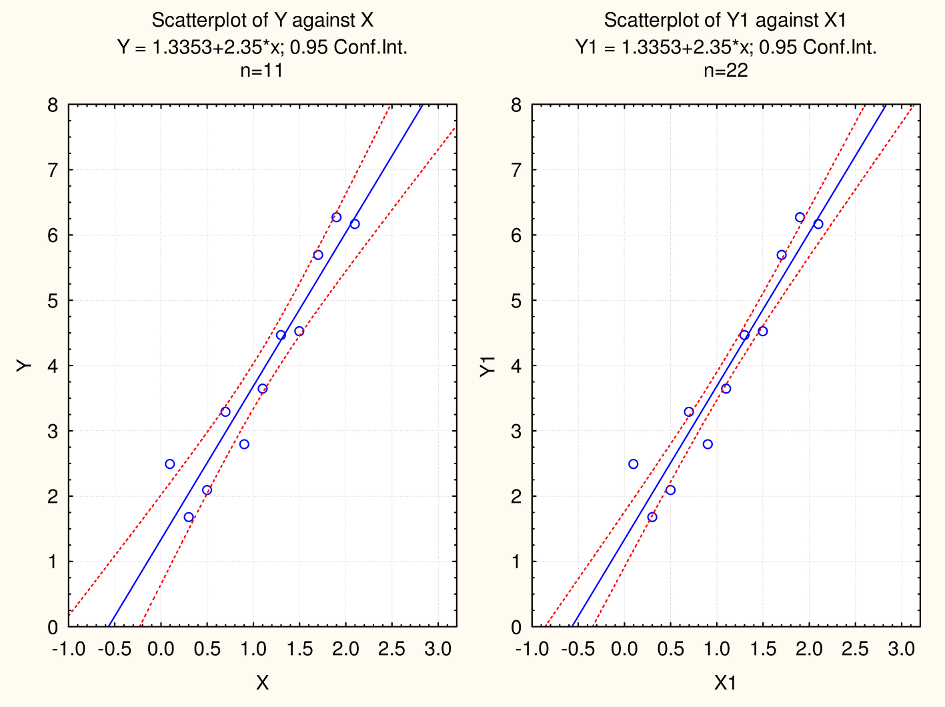
\includegraphics[scale=1.2]{6_regrConf.png}}
    {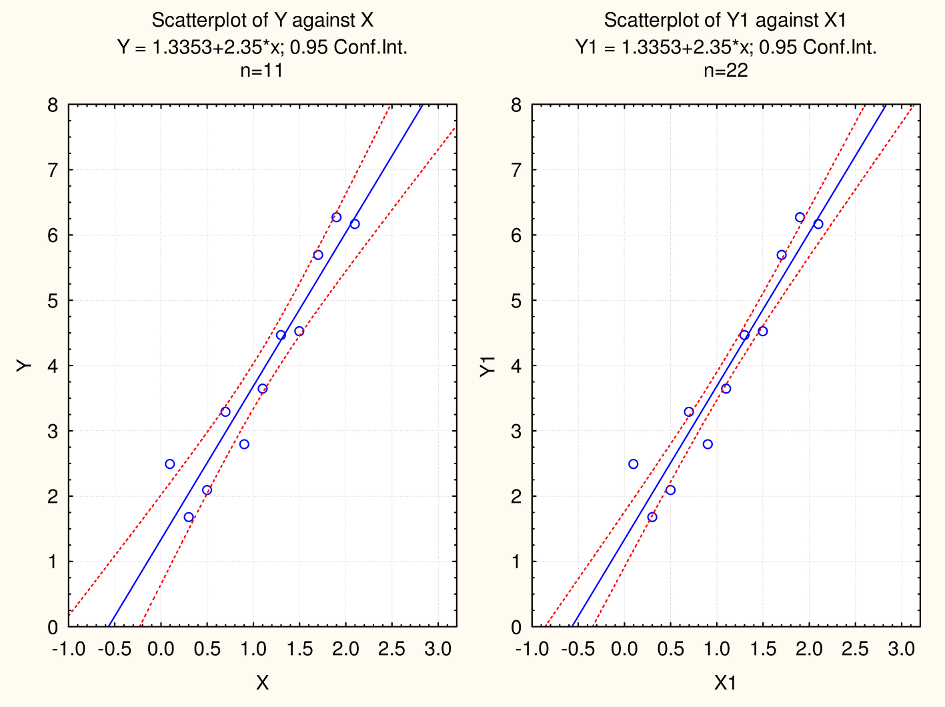
\includegraphics[scale=0.8]{6_regrConf.png}}
  \end{center}
\end{frame}

\livelloB{Prediction bands for the regression}

\begin{frame}
  \vspace*{.5cm}
  \begin{itemize}
    \item The confidence bands can be interpreted like the bands we expected that the ``real'' regression line, with a certain confidence degree, stands.
    \vspace*{.75cm}
    \item If we want to know (after having fixed the values of the independent variables) where it is expected that the potential future value of the y, we use the \textbf{prediction intervals (or bands)}.
  \end{itemize}
\end{frame}

\begin{frame}
  \vspace*{.25cm}
  \begin{itemize}
    \item As for the confidence bands, in a ``synthetic'' (matrix) mathematical form, it is possible to demonstrate that the limits of the prediction interval with level $(1-\alpha)$ for the regression curve, for a vector of explanatory (independent) variables $\underline{x}_*$ values, are: \\
      \vspace*{.1cm}
      LPL: $f(\underline{x}_*;\hat{\underline{\beta}})-t_{n-p-1;\,\frac{\alpha}{2}}\cdot \left[\sqrt{\underline{x}_*^T(X^TX)^{-1}\underline{x}_*+1}\right]\cdot \hat{\sigma_\varepsilon}$ \\
      \vspace*{.1cm}
      UPL: $f(\underline{x}_*;\hat{\underline{\beta}})+t_{n-p-1;\,\frac{\alpha}{2}}\cdot \left[\sqrt{\underline{x}_*^T(X^TX)^{-1}\underline{x}_*+1}\right]\cdot \hat{\sigma_\varepsilon}$ \\
      \vspace*{.1cm}
      where $\hat{\underline{\beta}}$ is the vector of the least squares parameters estimation and the operator $^T$ represents the matrix transposition.
    \vspace*{.25cm}
    \item The size of this interval, then, is equal to $2\cdot t_{n-p-1;\,\frac{\alpha}{2}}\cdot \left[ \sqrt{\underline{x}_*^T(X^TX)^{-1}\underline{x}_*+1} \right]\cdot \hat{\sigma_\varepsilon}$
    \vspace*{.25cm}
    \item It has to be noticed the strong ``similarity'' with the confidence intervals.
  \end{itemize}
\end{frame}

\begin{frame}
  \vspace*{.25cm}
  \begin{itemize}
    \item As the quantity $ \underline{x}_*^T(X^TX)^{-1}\underline{x}_* $ is often lesser than 1, the size of the prediction interval is quite always ``overlooked'' by the element ``+1'' within square brackets.
    \item The prediction bands, even though they have a ``similar'' behavior to those of the confidence bands, tend to be ``wider'' than the first ones, and to assume a less marked curvature than the one we highlighted before.
    \item The following plot shows the same regression lines of the previous graphic, with confidence band by  95\% (in red) and prediction bands by 95\% (in green). 
    \item It has to be noticed how the prediction bands seems to be ``parallel'' to the regression line. Furthermore, the prediction bands are wider than the confidence ones.
  \end{itemize}
\end{frame}

\begin{frame}
  \begin{center}
    \ifthenelse{\equal{\materiale}{jmp}}
    {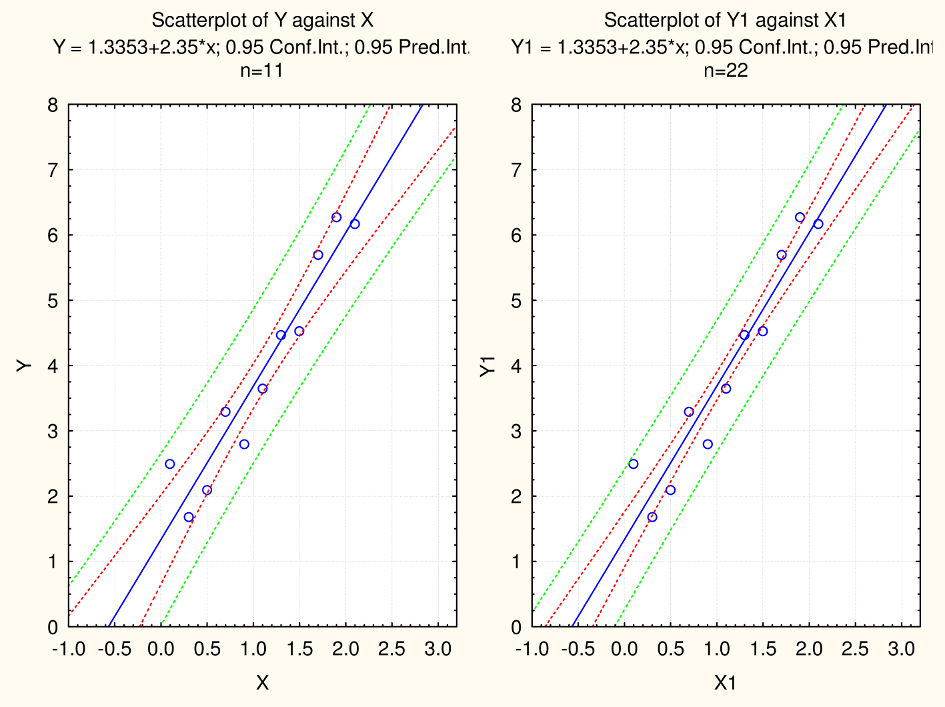
\includegraphics[scale=1.2]{6_regrPrev.png}}
    {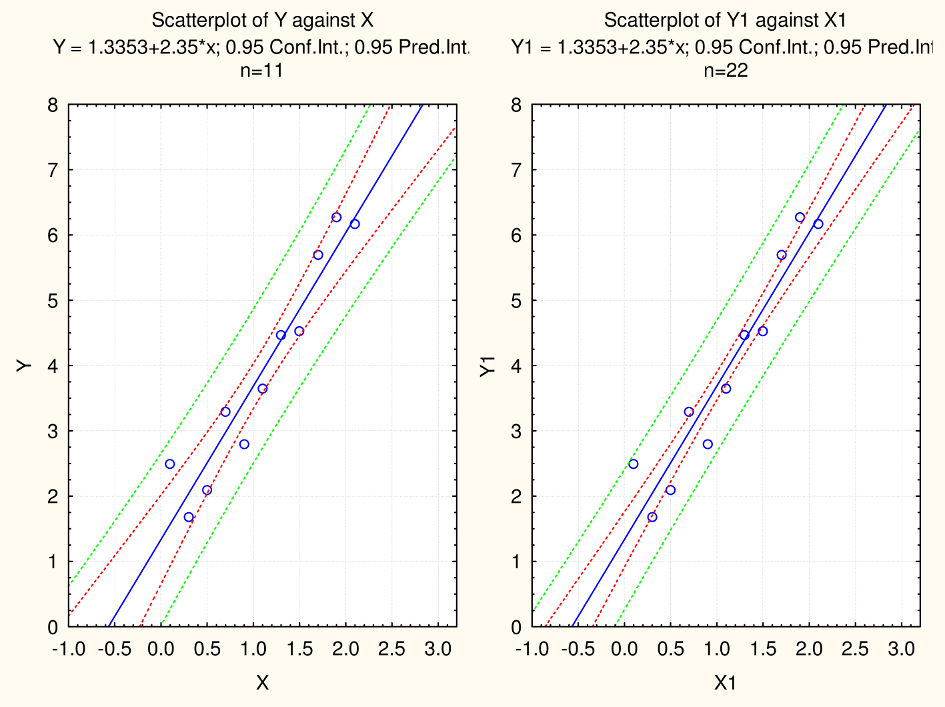
\includegraphics[scale=0.8]{6_regrPrev.png}}
  \end{center}
\end{frame}

\begin{frame}
  \vspace*{.25cm}
  \begin{itemize}
    \item We expect that the confidence bands tend to ``meet'' as the sample numorisity increases. On the contrary, this cannot happen for the prediction bands. 
    \vspace*{.25cm}
    \item This happens because the prediction bands express the variability of the single observations ($ y_i $).
    \vspace*{.25cm}
    \item If the specified regression model is correct, we will then expect that, about a fraction equal to $ \alpha $ of the future observations ``goes out'' from the prediction bands. 
    \vspace*{.25cm}
    \item This cannot be said for the confidence bands.
  \end{itemize}
\end{frame}



\livelloA{Analysis of covariance} 

\begin{frame}
  \begin{itemize}
    \item The analysis of the covariance, or \textbf{ANCOVA}, is a mix of the ANOVA and of the regression for quantitative variables.
    \vspace{0.2cm}
    \item In the ANCOVA a phenomenon is explained:
    \begin{itemize}
      \item by qualitative variables, the factors, as in the ANOVA;
      \item by quantitative variables called \textbf{covariate}.
    \end{itemize}
    \vspace{0.2cm}
    \item In the easiest case, the ANCOVA is used when it is identified another qualitative variable linked to the dependent variable, beyond the qualitative dependent variable.
    \vspace{0.2cm}
    \item If the link between the dependent variable and the covariate is strong, it is possible to extract the quota of variance due to the covariate from the $ MS_E $.
  \end{itemize}
\end{frame}

\begin{frame}
  The following plot shows two possible settings that can happen after using ANCOVA: \textbf{to emphasize the differences among the groups} (on the left) or \textbf{to exclude possible differences among groups} (on the right).\\
  \vspace{-.65cm}
  \begin{figure}
    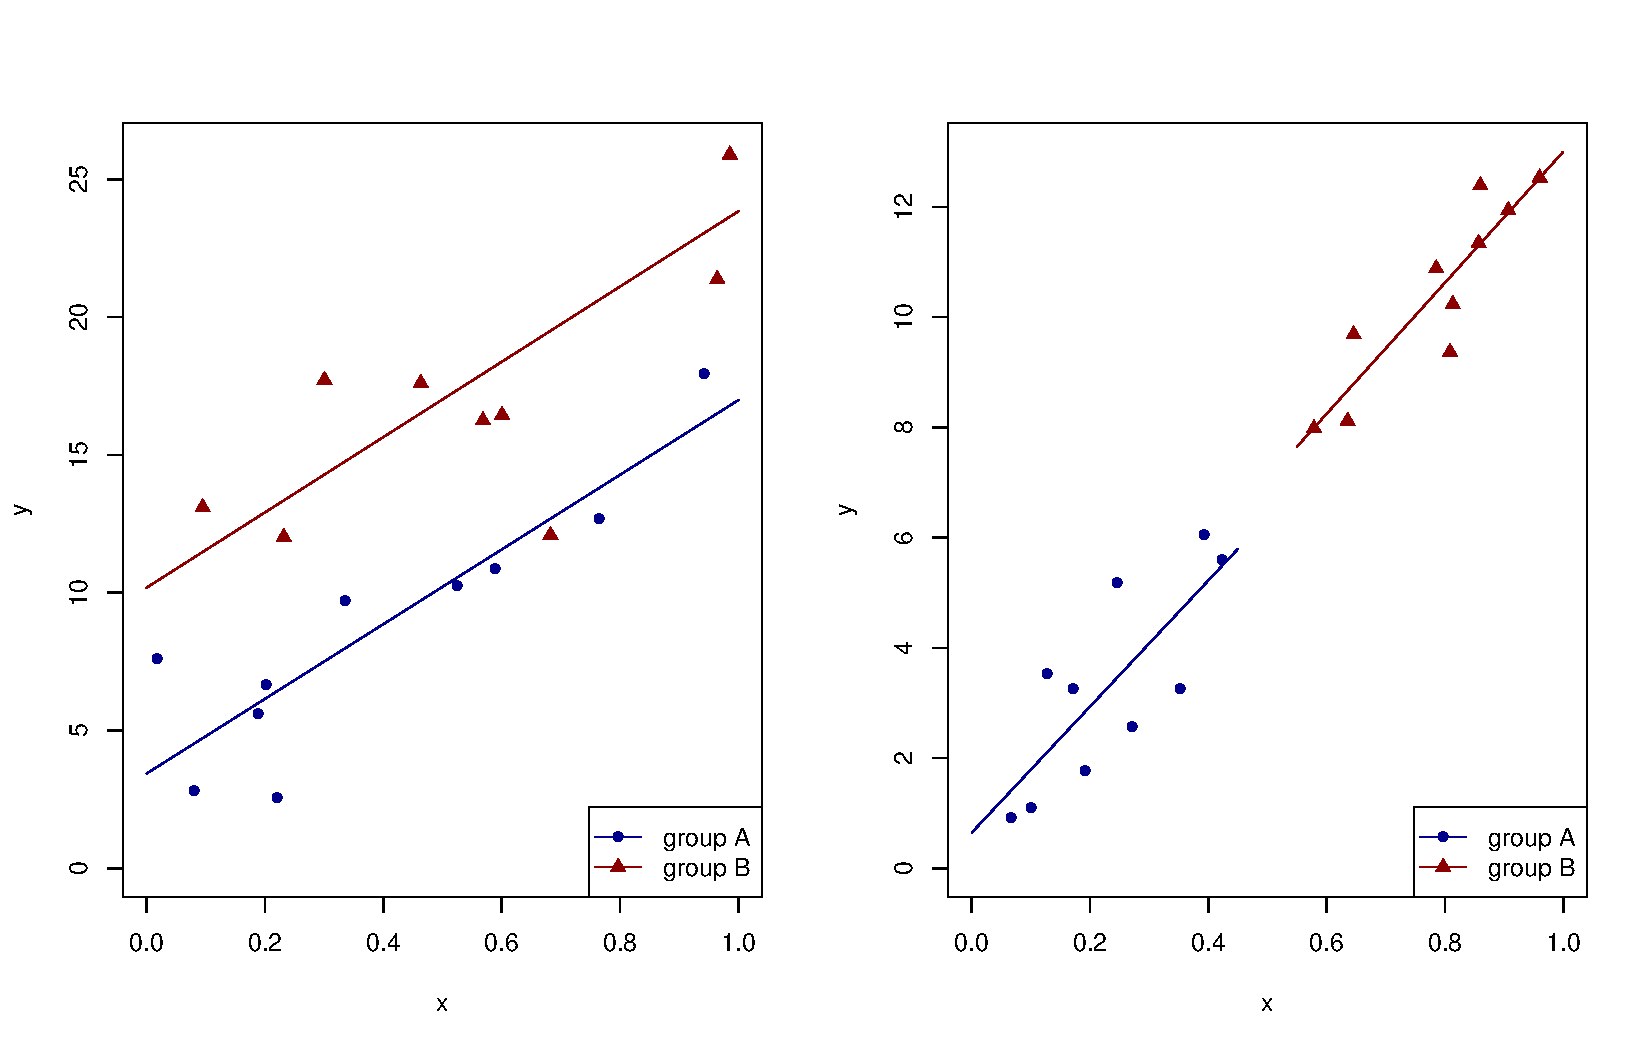
\includegraphics[scale=0.4]{6_ancova1.pdf}
  \end{figure}
\end{frame}

\begin{frame}
  \vspace{.25cm}
  \textbf{Example}.\\
  We want to determine if two hypnotic medicine, A and B, have the same effectiveness in making the patients being hypnotized.\\
  With this aim, we select 20 subjects:
  \begin{itemize}
    \item 10 subjects treated with the medicine A;
    \item 10 subjects treated with the medicine B.
  \end{itemize}
  The hypnothic suggestion is measured with a quantitative scale from 1 to 50 (the higher is the score, the higher is the suggestion).\\
  The effectiveness of hypnotic suggestion is subjective because it depends on the susceptibility of the patient. Before the administration of the medicine, the subjects have to do a susceptibility test. The higher is the score of the test, the higher is the susceptibility of the hypnosis.
\end{frame}

\begin{frame}
  If we analyse the data with an ANOVA whose model is
  \vspace{-0.2cm} $$ x_{ij} = \mu + \alpha_j + \varepsilon_{ij} $$
  we will obtain the following results:\\
  \vspace{0.3cm}
  \begin{center}
    \begin{tabular}{|c|c|c|c|c|c|}
      \hline
                  & $df$ & $SS$   & $MS$  & $F$    & $P(F)$  \\ \hline
      $Medicine$   & 1    & 6.05   & 6.05  & 0.1644 & 0.69    \\ \hline
      $residuals$ & 18   & 662.50 & 36.81 &        &         \\ \hline
      $Total$    & 19   & 668.55 &       &        &         \\ \hline
    \end{tabular}   
  \end{center}
  From the results of the ANOVA, there is no difference between the patients that have been treated with different medicines.\\
  In this model the susceptibility of the hypnotic suggestion, different in every subject, was not taken into consideration.
\end{frame}

\begin{frame}
  \vspace{.75cm}
   The analysis of the covariance is able to use the link between the hypnotic suggestion of the medicine and the susceptibility of the patient.\\
  \vspace{.50cm}
  The mathematical model is the following one:
  $$ x_{ij} = \mu + \alpha_j + \beta \cdot c_{ij} + \varepsilon_{ij} $$
  where $c_{ij}$ is the value that has been measured by the covariate (the susceptibility to the hypnotic suggestion) for the $ i $th subject of the $ j $th level.\\
\end{frame}

\begin{frame}
  \vspace{.25cm}
  If we analyse the relation between the dependent variable and the covariate one, we will obtain the following formula:
  \vspace{-0.3cm} $$ y = 17.9 + 0.7 \cdot x $$ \\
  \vspace{-0.5cm}
  \begin{figure}
    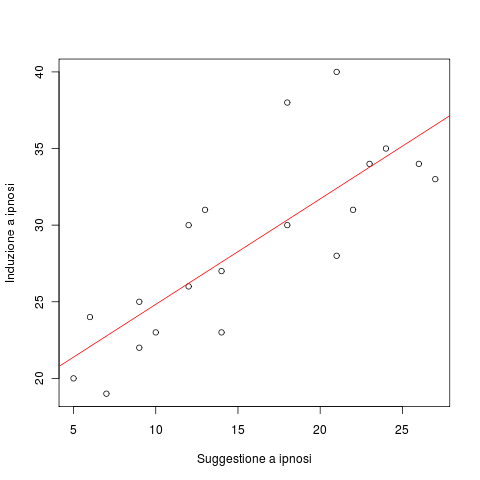
\includegraphics[height=4cm]{ancova_regressione.png}
  \end{figure}
  \vspace{-0.3cm}
  The model explains a part of the variance of the response variable (hypnosis induction). It is possible to identify, in the error variance, the element due to the covariate (hypnosis suggestion).
\end{frame}

\begin{frame}
  \begin{itemize}
    \item \textbf{ANOVA}
  \end{itemize}
  \begin{center}
    \begin{tabular}{|c|c|c|c|c|c|}
      \hline
                  & $df$ & $SS$   & $MS$  & $F$    & $P(F)$ \\ \hline
      $Medicine$   & 1    & 6.05   & 6.05  & 0.1644 & 0.69   \\ \hline
      $residuals$ & 18   & 662.50 & 36.81 &        &        \\ \hline
      $Total$    & 19   & 668.55 &       &        &        \\ \hline
    \end{tabular}\\
  \end{center}
  \begin{itemize}
    \item \textbf{ANCOVA}
  \end{itemize}
  \begin{center}
    \begin{tabular}{|c|c|c|c|c|c|}
      \hline
                    & $df$ & $SS$   & $MS$   & $F$    & $P(F)$    \\ \hline
      $Medicine$     & 1    & 6.05   & 6.05   & 0.8403 & 0.37      \\ \hline
      $suggestion$ & 1    & 540.18 & 540.18 & 75.07  & $<$0.0001 \\ \hline
      $residuals$   & 17   & 122.32 & 7.20   &        &           \\ \hline
      $Total$      & 19   & 668.55 &        &        &           \\ \hline
    \end{tabular}
  \end{center}
  \begin{itemize}
    \item The analysis of covariance shows that the $ SS_{suggestion} $ summed to the $ SS_{residuals} $ is equal to $ SS_{residuals} $ of the ANOVA.
  \end{itemize}
\end{frame}

\begin{frame}
  \vspace*{0.25cm}
  For the classic ANCOVA, it is necessary to demonstrate that the slope of the covariate does not significantly change when the treatment levels change.\\
  The following plot shows the regression lines for two kinds of medicine. 
  \vspace*{.15cm}
  \begin{figure}
    \centering
    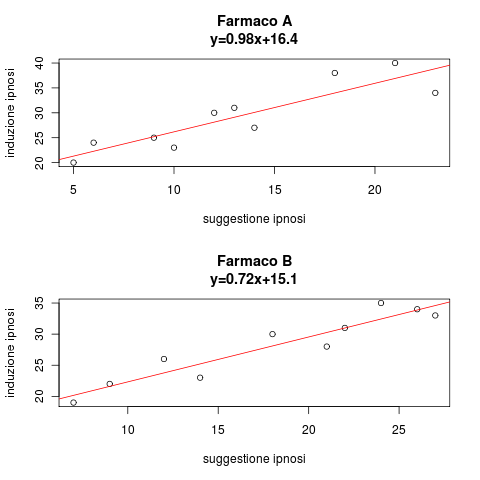
\includegraphics[height=5cm]{6_regAncova.png}\\
  \end{figure}
\end{frame}

\begin{frame}
  \vspace*{0.25cm}
  \begin{itemize}
    \item We can use a t test to check the equality of the slopes of the model in order to test the homogeneity of the slopes.
    \vspace{0.2cm}
    \item The null hypothesis, $ H_0 $, affirms that there is no difference between the coefficients of the various models. On the contrary, the alternative hypothesis, $ H_A $, affirms that there is difference.
    \vspace{0.2cm}
    \item The $ t $ value has to be calculated in order to verify or to refuse the null hypothesis:
      $$ t = \frac{\hat{\beta}_A - \hat{\beta}_B}{\sqrt{MSE_A + MSE_B}} $$\\
    \vspace{0.2cm}
    \item The index $ t $ has to be compared to the cut-off value of the Student's t distribution: $ t \sim t_{n_A+n_B-4} $.
  \end{itemize}
\end{frame}





\end{document}
